\documentclass[../main/main.tex]{subfiles}

\raggedbottom

\makeatletter
\renewcommand{\@chapapp}{M\'ecanique -- chapitre}
\makeatother

% \toggletrue{student}

\begin{document}
\setcounter{chapter}{3}

\chapter{Approche \'energ\'etique du mouvement}

\section{Notions énergétiques}
\subsection{Énergie}
L’énergie est un concept physique très puissant et présent dans tout les
domaines de la physique mais qu’il est difficile de définir simplement. En voici
une première définition qualitative~:
\begin{tdefi}{Définition~: énergie, sidebyside, righthand ratio=.3}
    L’énergie d’un système est sa capacité à agir sur lui-même ou d’autres
    systèmes.
    \tcblower
    Unité~: le \textbf{Joule} (J)
\end{tdefi}

Ainsi, le mouvement d'un corps, les échanges de chaleur, les courants
électriques et tous les phénomènes physiques résultent d'échanges d'énergie.
Elle respecte une propriété principale, fondamentale de l'approche du monde qui
nous entoure~:

\begin{tprop}{Propriété~: conservation de l'énergie, halign=center}
    \bfseries
    L’énergie est une grandeur conservative. Elle ne peut être créée ou
    détruite. Elle ne peut que changer de forme et/ou passer d’un système à un
    autre.
\end{tprop}

Ces notions serons retravaillées en thermodynamique.

\vspace{-10pt}
\subsection{Puissance}

Une énergie totale peut varier différemment selon les conditions du système, et
notamment varier plus ou moins vite. Cette variation est une information
caractéristique de l'évolution d'un système~: une voiture qui freine pour
diminuer son énergie cinétique peut le faire lentement ou rapidement et
donnerons des ressentis physiques très différents. On définit pour ça la
puissance d'une énergie~:

\begin{tdefi}{Puissance, sidebyside}
    La \textbf{puissance} $\Pc$ d'une énergie $\Ec$ traduit sa \textbf{variation
    temporelle}, et on a
    \[\boxed{\Pc = \dv{\Ec}{t}}\]
    \tcblower
    L'unité d'une puissance est donc homogène à des \si{J.s^{-1}}, et se compte
    couramment en \textbf{Watts} (W). On a
    \[\boxed{\SI{1}{W} = \SI{1}{J.s^{-1}}}\]
\end{tdefi}

\vspace{-10pt}
\section{Énergie cinétique et travail d'une force constante}
\subsection{Énergie cinétique}

\begin{tdefi}{Définition~: énergie cinétique, sidebyside}
    Un point matériel M de masse $m$ allant à la vitesse $v$ dans un référentiel
    galiléen $\Rc$ a pour énergie cinétique~:
    \[\boxed{\Ec_{c}\Rg(\Mr) = \frac{1}{2}mv\Rg(\Mr)^2}\]
    \tcblower
    L'unité d'une énergie est en \fbox{\textbf{joules}} (J), et dépend du référentiel.
\end{tdefi}

\subsection{Travail d'une force}

\textbf{À quelle condition une force appliquée à un objet fait-elle varier son
énergie cinétique~?}
\begin{itemize}
    \item Quand un objet est jeté vers le haut, le poids le ralentit, donc fait
        diminuer son énergie cinétique.
    \item Quand un objet tombe, le poids l’accélère et fait donc augmenter son
        énergie cinétique.
    \item Lorsqu’un objet est posé sur un support, la réaction normale ne fait
        pas varier son énergie cinétique.
    \item Lorsqu’un objet freine sur un support horizontal, la réaction normale
        ne cause pas la variation de son énergie cinétique (c’est la réaction
        tangentielle qui le freine).
\end{itemize}
\textbf{Le travail est une grandeur physique construite pour rendre compte de
l’effet d’une force sur son énergie cinétique.}
\begin{itemize}
    \item En l’absence de déplacement, le travail doit être nul.
    \item Si la force est perpendiculaire au déplacement, le travail doit être
        nul.
    \item Si la force est dans le sens du déplacement, le travail doit être
        positif et maximal.
    \item Si la force est dans le sens opposé au déplacement, le travail doit
        être négatif (et minimale).
\end{itemize}

\begin{tdefi}{Définition~: travail d'une force constante, sidebyside, heart}
    Le travail $W_{\ABr}$ d'une force \textbf{constante} $\Ff$ sur un chemin $\AB$ est
    \[\boxed{W_{\ABr}(\Ff) = \Ff\cdot\AB}\]
    où «~$\cdot$~» désigne le produit scalaire entre deux vecteurs.
    \tcblower
    Un \textbf{travail} est homogène à une \textbf{énergie}, donc s'exprime en
    \fbox{\textbf{joules}}.
\end{tdefi}

\begin{rrema}{Remarques}
    \begin{itemize}
        \item Si $W_{\ABr} > 0$, on dit que le travail est \textbf{moteur}~; si
            $W_{\ABr} < 0$ il est \textbf{résistant}.
        \item $W_{\ABr} = 0 \Ra$ soit $\Ff = \of$, soit $\AB = \of$, soit
            $\AB\perp\Ff$.
    \end{itemize}
\end{rrema}

\subsection{Exemples de travaux}

On peut calculer un travail avec deux formes mathématiques équivalentes~:
\begin{itemize}
    \item En utilisant une base de projection, \textit{par exemple} cartésienne,
        on décompose la force et le déplacement~:
        \[
            \Ff = F_x\ux + F_y\uy + F_z\uy
                = \mqty(F_x\\F_y\\F_z)
            \qet
            \AB = x\ux + y\uy + z\uz
                = \mqty(x\\y\\z)
        \]
        On a alors
        \[
            \boxed{\Ff\cdot\AB = xF_x + yF_x + zF_z}
            =
            \mqty{\\+\\+}
            \mqty(F_x\\F_y\\F_z)
            \mqty{\times\\\times\\\times}
            \mqty(x\\y\\z)\]
    \item En utilisant une autre définition du produit scalaire~:
        \[\boxed{\Ff\cdot\AB = \norm{\Ff}\times\norm{\AB}\cos\a}\]
        avec $\a$ l'angle entre les vecteurs.
\end{itemize}

\begin{rexem}{Application}
    On a vu en TD qu'un objet, de vitesse initiale $v_0\ux$, soumis à une force
    de frottements solides sur un support horizontal subissait, lors de son
    mouvement avec glissement,
    \[\Ff = -fmg\ux\]
    et parcourait pendant la phase de freinage la distance
    \[D = \frac{v_0{}^2}{2fg}\]
    \textbf{Calculer le travail de la force de frottements sur cette distance}.
    Est-il moteur ou résistant~?
    \tcblower
    \cswitch{white}{
        \begin{align*}
            W_{\ABr}(\Ff) &= \Ff\cdot\AB
            \\\Lra
            W_{\ABr}(\Ff) &= \norm{\Ff}\times\norm{\AB}\times\cos(\pi)
            \\\Lra
            W_{\ABr}(\Ff) &= fmg\times\frac{v_0{}^2}{2fg}\times(-1)
            \\\Lra
            \Aboxed{W_{\ABr}(\Ff) &= - \frac{1}{2}mv_0{}^2}
        \end{align*}
        Le travail étant négatif, on dit qu'il est (et que la force est)
        \textbf{résistant}(e). On observe que l'énergie initiale du système, son
        énergie cinétique, a été dissipée par la force de frottements.
    }
\end{rexem}

\begin{rexem}{Application}
    Calculer le travail du poids lors d'un déplacement avec changement
    d'altitude.
    \tcblower
    \begin{minipage}{0.20\linewidth}
        \begin{center}
            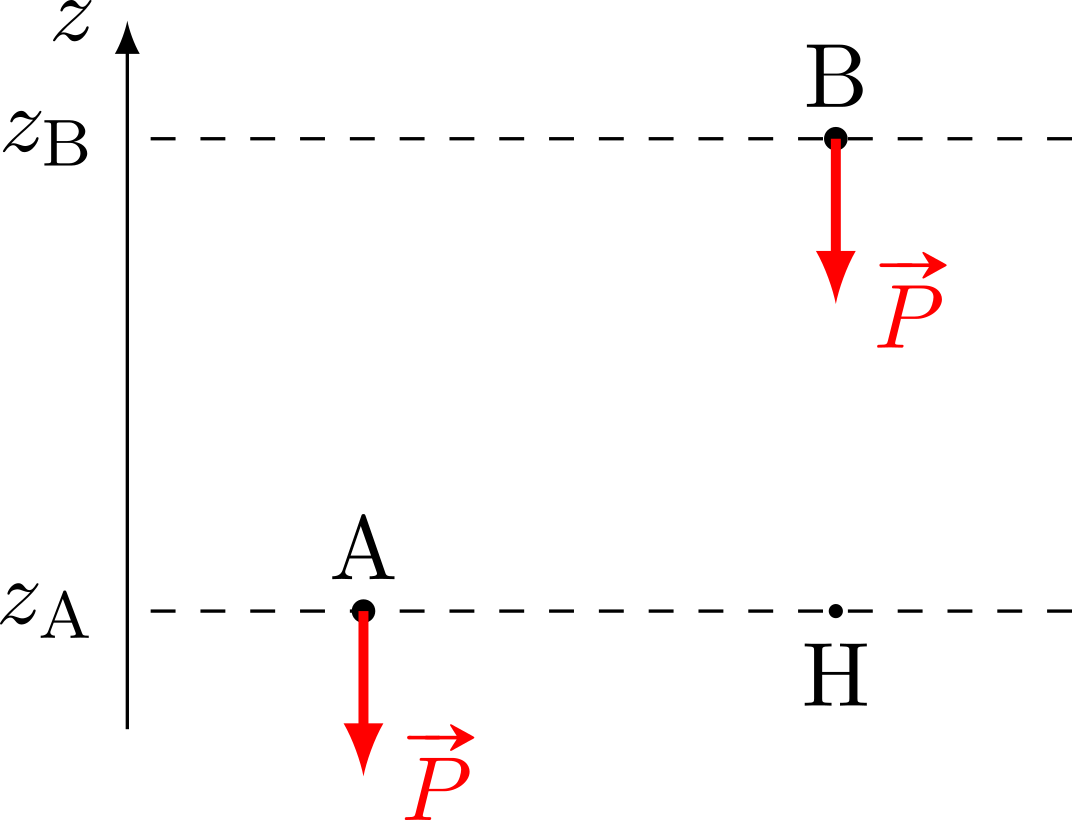
\includegraphics[width=\linewidth]{w_p}
        \end{center}
    \end{minipage}
    \hfill
    \begin{minipage}{.75\linewidth}
        \[W_{\ABr}(\Pf) = \Pf\cdot\AB\]
        En projection cartésienne~:
        \begin{gather*}
            \Pf = -mg\uz
            \qet
            \AB = (x_\Br-x_\Ar)\ux + (y_\Br - y_\Ar)uy + (z_\Br - z_\Ar)\uz
            \\
            W_{\ABr}(\Pf) = -mg(z_\Br - z_\Ar)
        \end{gather*}
    \end{minipage}
\end{rexem}

\begin{tprop}{Propriété~: travail du poids, hand}
    Le travail du poids entre un point A et un point B est~:
    \[\boxed{W_\ABr(\Pf) = mg(z_\Ar - z_\Br)}\]
\end{tprop}

\begin{rexem}{Application}
    On considère une voiture allant d'un point A à un point B, éloignés de
    \SI{100}{km}, avec une vitesse constante. La force de frottement exercée par
    l'air est
    \[\Ff = -\frac{1}{2}\rho Sc_xv\vf\]
    Déterminer son travail, et faire l'application
    numérique pour $v = \SI{50}{km.h^{-1}}$ puis \SI{80}{km.h^{-1}}. On donne $S
    = \SI{3.07}{m^2}$, $c_x = \num{0.33}$, $\rho = \SI{1.3}{kg.m^{-3}}$. 
    \tcblower
    \begin{minipage}{0.45\linewidth}
        \begin{center}
            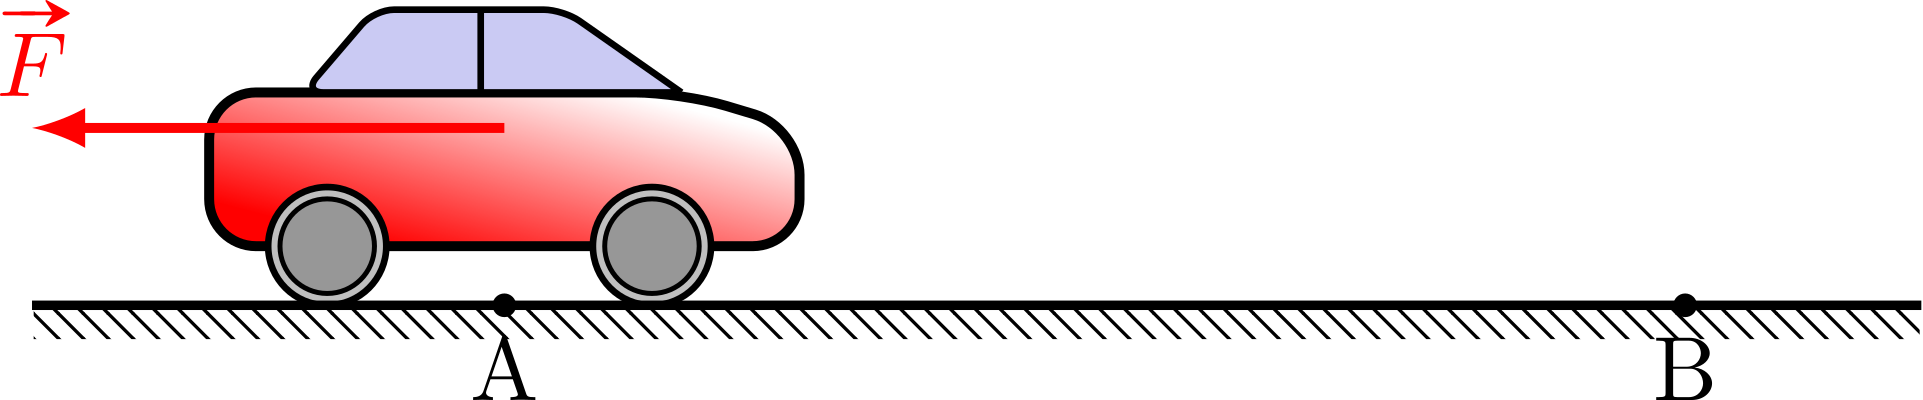
\includegraphics[width=\linewidth]{voiture}
        \end{center}
    \end{minipage}
    \hfill
    \begin{minipage}{0.45\linewidth}
        \[W_{\ABr}(\Ff) = \Ff\cdot\AB = -F\times\ABr\]
        Le travail est négatif, la force est résistante.
        \begin{itemize}
            \item $v = \SI{50}{km.h^{-1}} \Ra W_{\ABr}(\Ff) = \SI{-1.27e7}{J}$,
                soit $\approx \SI{0.4}{L}$ d'essence~;
            \item $v = \SI{80}{km.h^{-1}} \Ra W_{\ABr}(\Ff) = \SI{-3.25e7}{J}$,
                soit $\approx \SI{1}{L}$ d'essence.
        \end{itemize}
    \end{minipage}
\end{rexem}

Ainsi, dans certains cas le travail ne dépend pas que du point de départ et
d'arrivée, mais peut dépendre de la \textbf{façon} d'y aller (vitesse, chemin
suivi…). En realité,
\begin{tror}{, halign=center}
    De façon générale, le travail dépend du chemin suivi.
\end{tror}

\subsection{Théorème de l'énergie cinétique}

\begin{tprop}{Théorème de l'énergie cinétique, heart}
    Dans un référentiel galiléen $\Rc$, un point matériel M de masse $m$,
    d'énergie cinétique $\Ec_c\Rg$ et subissant les forces extérieures $\Ff_i$
    sur la distance AB vérifie
    \[\boxed{\D_{\ABr}\Ec_c\Rg = \Ec(\Br) - \Ec(\Ar) = \sum_i W_{\ABr}(\Ff_i)}\]
\end{tprop}

\begin{rexem}{Application}
    Déterminer la vitesse d'une skieuse en bas d'une piste de $h = \SI{5}{m}$ de
    dénivelé partant avec une vitesse nulle, si on néglige les frottements.
    \tcblower
    \cswitch{white}{
        \begin{itemize}
            \item $\D\Ec_{c}\Rg$~: l'énergie cinétique initiale est nulle en supposant
                une vitesse initiale nulle~; en bas de la piste, on a la vitesse
                $v$, soit
                \[\D\Ec_c\Rg = \frac{1}{2}mv^2 - 0 = \frac{1}{2}mv^2\]
            \item $W_{\ABr}(\Ff_i)$~: la réaction de la piste est
                perpendiculaire au mouvement, donc son travail est nul. Pour le
                poids, on a
                \[W_{\ABr}(\Pf) = mg(z_\Ar - z_\Br) = mgh\]
        \end{itemize}
        Ainsi, avec le TEC entre le haut et le base de la piste, on a
        \[
            \frac{1}{2}mv^2 = mgh
            \quad\Ra\quad
            \boxed{v = \sqrt{2gh} = \SI{10}{m.s^{-1}}}
        \]
    }\vspace*{-20pt}
\end{rexem}

\subsection{Quand utiliser une approche énergétique~?}

\begin{itemize}
    \item Si l’on veut connaître seulement une vitesse / une distance à la fin
        d’un processus (chute, descente, freinage, etc.), les méthodes
        énergétiques sont souvent plus simples et plus rapides.

    \item Si on cherche les équations horaires / un temps / une trajectoire, il
        faut appliquer le PFD.
\end{itemize}

Dans tous les cas, ça donne le même résultat~!

\section{Puissance d'une force et théorème de la puissance cinétique}
\subsection{Définition}
Si la puissance est en effet la dérivée d'une énergie par rapport au temps, on
peut l'exprimer comme étant la rapidité avec laquelle un travail (homogène à une
énergie) peut être effectué. La puissance moyenne ainsi définie comme
\[\Pc_m = \frac{W_{\ABr}}{\Dt}\]

Comme pour la vitesse et l'accélération, on définit cette grandeur sur un temps
infinitésimal~:

\begin{tdefi}{Définition~: puissance instantanée d'une force, sidebyside, heart}
    On définit la \textbf{puissance instantanée} d'une force $\Ff$ comme étant~:
    \[\boxed{\Pc\Rg(\Ff) = \Ff\cdot\vf\Rg}\]
    \tcblower
    % \begin{center}
    %     \color{deficol}\bfseries
    %     Unité~:
    % \end{center}
    Elle dépend du référentiel, et s'exprime en \textbf{watts} (W).
\end{tdefi}

\begin{rexem}{Application}
    Calculer la puissance du poids lors d'une descente à vélo d'une pente
    d'angle $\a$.
    \tcblower
    \begin{minipage}{0.35\linewidth}
        \begin{center}
            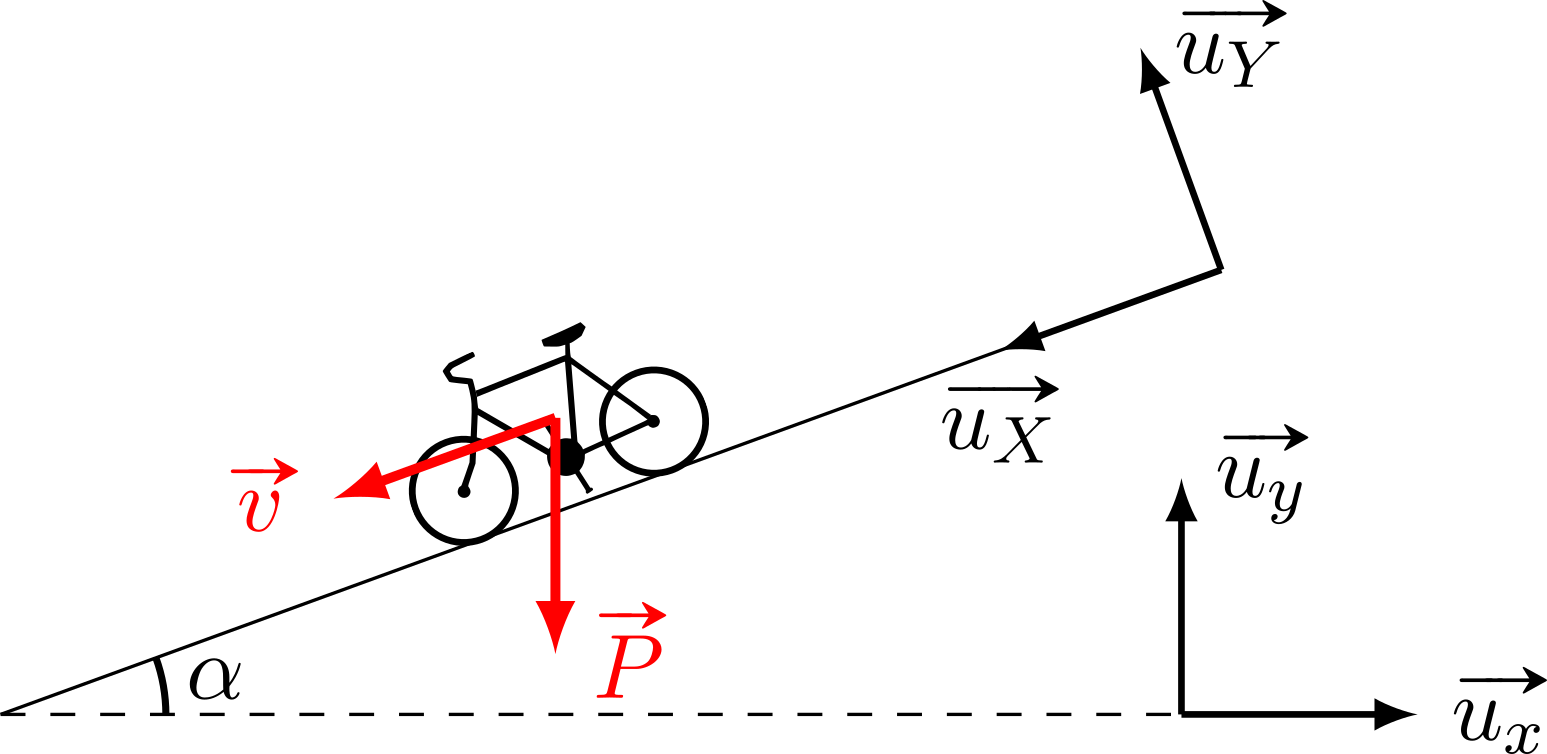
\includegraphics[width=\linewidth]{velo}
        \end{center}
    \end{minipage}
    \hfill
    \begin{minipage}{0.60\linewidth}
        Dans la base $(\vv{u_X},\vv{u_Y})$~:
        \begin{gather*}
            \Pf = m\gf = mg(-\cos\a\vv{u_Y} + \sin\a\vv{u_X})
            \\\text{et}\quad
            \vf = v\vv{u_X}
        \end{gather*}
        Ainsi, dans le référentiel de la route~:
    \end{minipage}\bigbreak
    \[\boxed{\Pc(\Pf) = \Pf\cdot\vf = mgv\sin\a}\]
    Dans ce cas, la puissance du poids est positive~: le poids en
    moteur. Dans le cas de la montée, on inverse le sens de $\vf$, et le poids
    devient résistant. \bigbreak
    On aurait pu obtenir ce résultant et remarquant que l'angle entre $\vf$ et
    $\Pf$ et $\pi/2-\a$, et utiliser $\cos(\pi/2-\a) = \sin\a$.
\end{rexem}

\vspace{-20pt}
\subsection{Théorème de la puissance cinétique}

\begin{tprop}{Théorème de la puissance cinétique, heart}
    Dans un référentiel galiléen $\Rg$, la variation instantanée de l'énergie
    cinétique d'un point matériel M est égale à la somme des puissances de
    forces qui s'exercent sur ce point~:
    \[\boxed{\dv{\Ec_c\Rg(\Mr)}{t} = \sum_i \Pc\Rg(\Ff_i)}\]
\end{tprop}

% \begin{rdemo}{Démonstration}
%     Différentes démonstrations sont possibles, soit en faisant un bilan de
%     puissance (c'est-à-dire PFD$\times\vf$), soit en partant de la définition de
%     l'énergie cinétique~:
%     \begin{rsidedemo}
%         \vspace{-10pt}
%         \begin{align*}
%             m\af &= \sum_i \Ff_i
%             \\\Lra
%             m \dv{v}{t}\cdot\vf &= \sum_i \Ff_i\cdot\vf
%             \\\Lra
%             \dv{t}(\frac{1}{2}mv^2) &= \sum_i \Pc(\Ff_i)
%             \\\Lra
%             \Aboxed{\dv{\Ec_c\Rg(\Mr)}{t} &= \sum_i \Pc\Rg(\Ff_i)}
%         \end{align*}
%         \tcblower
%         \vspace{-10pt}
%         \begin{align*}
%             \dv{\Ec_c}{t} &= \dv{t}(\frac{1}{2}m\vf\cdot\vf)
%             \\
%                           &= \frac{1}{2}m \left( \vf\cdot \dv{\vf}{t} + \dv{\vf}{t}
%                           \cdot \vf\right)
%             \\
%                           &= m\dv{\vf}{t}\cdot\vf
%             \\\Lra
%             \dv{\Ec_c}{t} &= \left( \sum_i \Ff_i \right)\cdot\vf
%         \end{align*}
%     \end{rsidedemo}
% \end{rdemo}

\begin{rdemoside}{Démonstration}
    \begin{center}
        \fbox{\textbf{Bilan de puissance}}
    \end{center}
    \vspace*{-15pt}
    \begin{align*}
        m\af &= \sum_i \Ff_i
        \\\Lra
        m \dv{\vf}{t}\cdot\vf &= \sum_i \Ff_i\cdot\vf
        \\\Lra
        \dv{t}(\frac{1}{2}mv^2) &= \sum_i \Pc(\Ff_i)
        \\\Lra
        \Aboxed{\dv{\Ec_c\Rg(\Mr)}{t} &= \sum_i \Pc\Rg(\Ff_i)}
    \end{align*}
    \tcblower
    \begin{center}
        \fbox{\textbf{Définition de $\Ec_c$}}
    \end{center}
    \vspace*{-15pt}
    \begin{align*}
        \dv{\Ec_c}{t} &= \dv{t}(\frac{1}{2}m\vf\cdot\vf)
        \\
                      &= \frac{1}{2}m \left( \vf\cdot \dv{\vf}{t} + \dv{\vf}{t}
                      \cdot \vf\right)
        \\
                      &= m\dv{\vf}{t}\cdot\vf
        \\\Lra
        \dv{\Ec_c}{t} &= \left( \sum_i \Ff_i \right)\cdot\vf
    \end{align*}
\end{rdemoside}


\begin{rexem}{Application}
    Justifier que les frottements conduisent à une baisse de l'énergie
    cinétique.
    \tcblower
    Les frottements sont dans la direction opposée à la vitesse, donc leur
    puissance est négative. La dérivée de l'énergie cinétique étant égale à la
    somme des puissances des forces est donc négative~: l'énergie cinétique
    décroît.
\end{rexem}

\begin{rexem}{Application}
    Établir l'équation différentielle du pendule.
    \tcblower
    \begin{minipage}{0.25\linewidth}
        \begin{center}
            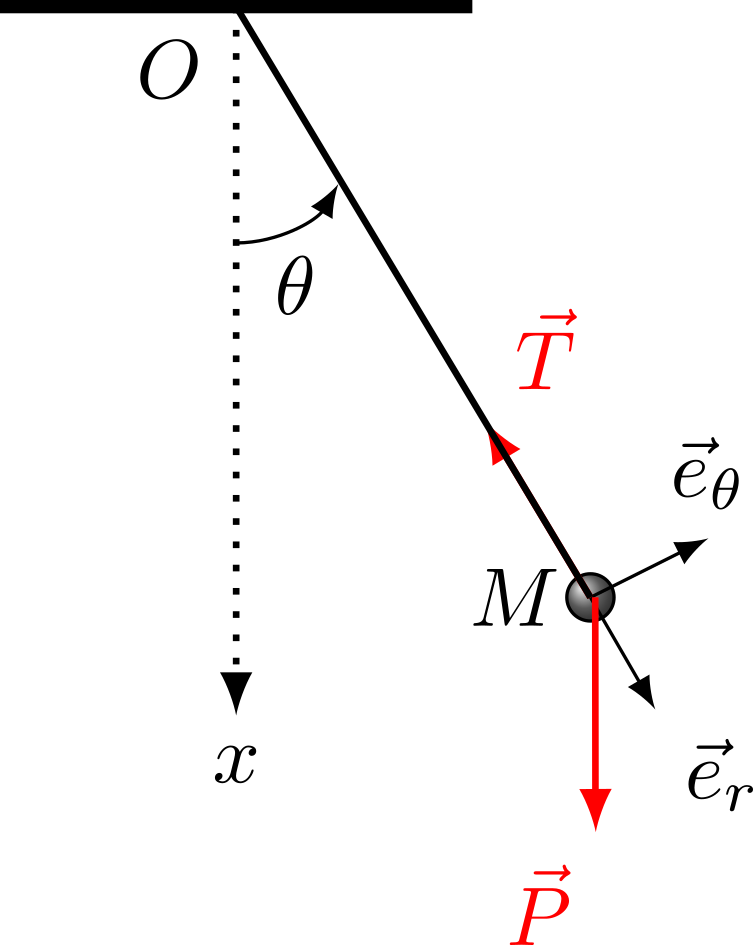
\includegraphics[width=\linewidth]{pendule_plain}
        \end{center}
    \end{minipage}
    \hfill
    \begin{minipage}{0.70\linewidth}
        Le mouvement étant circulaire, $\vf = \ell\tp\ut$ et on a
        \[\Ec_c = \frac{1}{2}m\ell^2\tp^2\]
        Ainsi,
        \[\dv{\Ec_c}{t} = m\ell^2\tp\tpp\]
        De plus, $\vf\perp\Tf$ et l'angle entre $\vf$ et $\Pf$ est $\pi/2+\tt$~:
        \[
            \Tf\cdot\vf = 0
            \qet
            \Pf\cdot\vf = mg\times\ell\tp\times\cos(\frac{\pi}{2}+\tt) =
            -mg\ell\tp\sin\tt
        \]
    \end{minipage}
    Avec le TPC,
    \[m\ell^2\tp\tpp = 0 - mg\ell\tp\sin\tt\]
    et en simplifiant par $m\ell^2\tp$~:
    \[\boxed{\tpp + \frac{g}{\ell}\sin\tt = 0}\]
\end{rexem}

\subsection{Quand appliquer le TPC~?}
\begin{itemize}
    \item Si le mouvement est \textbf{selon une coordonnée} ($x$, $y$ ou $z$ en
        cartésiennes, $\tt$ en coordonnées cylindriques), il est pertinent
        d'utiliser le TPC.
    \item Sinon (chute libre avec angle par exemple), on revient au PFD qui
        contient toute l'information.
\end{itemize}

\section{Travail élémentaire}
\subsection{Définition}
La variation d'énergie cinétique due à une force $\Ff$ pendant un temps
infinitésimal $\dt$ est, d'après le TPC~:

\[\dd\Ec_c = \sum \Ff\cdot\vf\dt\]
On retrouve le déplacement élémentaire $\dd{\OM} = \vf\dt$. Ainsi, ayant deux
énergies à gauche et à droite, on définit~:

\begin{tdefi}{Définition~: travail élémentaire, heart}
    Le travail élémentaire $\de W$ d'une force $\Ff$ sur un déplacement
    infinitésimal $\dd\OM$ est~:
    \[\boxed{\de W = \Ff\cdot\dd\OM}\]
\end{tdefi}

\begin{timpo}{Attention, hand}
    Il ne faut pas confondre la notation $\de$ et la notation $\dd$. \bigbreak
    La notation $\de$ fait référence au fait que le travail total dépend
    \textit{a priori} du chemin suivi et de la vitesse à laquelle on parcourt ce
    chemin, et non pas uniquement du point de départ et du point d'arrivée. Un
    travail se définit sur une \textbf{distance}, pas
    \cancel{\bcancel{\textbf{en un point}}}. On peut écrire~:

    \[
        \int_\Ar^\Br \dd\Ec_c = \Ec_c(\Br) - \Ec_c(\Ar)
        \qet
        \int_\Ar^\Br \dd\OM = \vec{\rm OB} - \vec{\rm OA} = \AB
    \]
    mais il est absurde d'écrire
    \[\cancel{\bcancel{
        \int_{\Ar}^{\Br} \de W = W(\Br) - W(\Ar)
        }}
    \]
\end{timpo}

\begin{tprop}{Propriété}
    Le travail d'une force sur un chemin AB se déduit du travail inifitésimal
    par~:
    \[\boxed{W_{\ABr}(\Ff) = \int_{\Ar}^{\Br} \de W}\]
\end{tprop}

\subsection{Exemples}
\subsubsection{Poids}
On a
\[
    \Pf = -mg\uz
    \qet
    \dd\OM = \dd{x}\ux + \dd{y}\uy + \dd{z}\uz
\]
D'où $\de W = -mg\dd{z}$ et
\[W_{\ABr} = \int_{\Ar}^{\Br} \de W = -mg \int_{\Ar}^{\Br} \dd{z}\]
et ainsi, on retrouve le résultat précédent~:
\[\boxed{W_{\ABr}(\Pf) = mg(z_\Ar - z_\Br)}\]

\subsubsection{Force de rappel élastique}
\[
    \Ff_r = -k(x-\ell_0)\ux
    \qet
    \dd\OM = \dd{x}\ux + \dd{y}\uy + \dd{z}\uz
\]
D'où $\de W = -k(x-\ell_0)\dd{x}$ et
\begin{gather*}
    W
        = \int_{\Ar}^{\Br} \de W
        = -k \int_{\Ar}^{\Br} (x-\ell_0)\dd{x}
        = -k \left[ \frac{1}{2}(x-\ell_0)^2 \right]_{\Ar}^{\Br}
    \\\Lra
    \boxed{W = -\frac{1}{2}k \left( (x_\Br - \ell_0)^2 - (x_\Ar
        -\ell_0)^2\right)}
\end{gather*}

\subsection{TEC}
On peut alors démontrer le TEC~:

\begin{rdemo}{Démonstration}
    \begin{gather*}
        \dd{\Ec_c} = \sum_i\Ff_i\cdot\vf\dt = \sum_i \Ff_i\cdot\dd\OM
        \\\Ra
        \int_{\Ar}^{\Br} \dd{\Ec_c} = \int_{\Ar}^{\Br} \sum_i \Ff_i\cdot\dd\OM
            = \sum_i \int_{\Ar}^{\Br} \Ff_i\cdot\dd\OM
        \\\Lra
        \D_{\ABr}\Ec_c = \sum_i \int_{\Ar}^{\Br} \de W_i
        \\\Lra
        \boxed{\D_{\ABr}\Ec_c = \sum_i W_{\ABr}(\Ff_i)}
    \end{gather*}
\end{rdemo}

\section{Énergie potentielle et énergie mécanique}
\subsection{Forces conservatives et non-conservatives}
Comme on l'a vu, le travail \textbf{peut} dépendre du chemin suivi. Dans le cas
du poids ou de la force de rappel, nous voyons que le travail ne dépend
cependant que des coordonnées des points de départ et d'arrivée~; ce sont des
forces particulières à cet égard, d'où la définition~:

\begin{tdefi}{Définition}
    Une force est dite \textbf{conservative} si son travail de A à B ne dépend pas du
    \underline{chemin} suivi ou de la vitesse, mais uniquement des
    \textbf{positions A et B}. Elle est \underline{non-conservative} dans le cas
    contraire.
\end{tdefi}

\begin{rexem}{Exemples}
    \begin{minipage}{0.45\linewidth}
        \textbf{Forces conservatives}~:
        \begin{itemize}
            \item Le poids~;
            \item La force de rappel d'un ressort~;
            \item La force gravitationnelle~;
            \item La force électrostatique.
        \end{itemize}
    \end{minipage}
    \hfill
    \begin{minipage}[b]{0.45\linewidth}
        \textbf{Forces non-conservatives}~:
        \begin{itemize}
            \item Frottement fluide~;
            \item Frottement solide…
        \end{itemize}
    \end{minipage} \bigbreak
    Tous les frottements sont non-conservatifs, puisqu'en faisant un détour
    pour aller de A à B, les frottements s'exerceront plus longtemps et donc
    la valeur du travail effectué sera plus élevé.
\end{rexem}

\subsection{Énergie potentielle}
Dans le cas d'une force conservative, on remarque qu'on peut donc légitimement
l'écrire avec une forme différentielle $\dd$ plutôt qu'avec $\de$, définissant
l'\textbf{énergie potentielle} d'une force~:
\begin{tdefi}{Définition, heart}
    À une force \textbf{conservative} $\Ff\ind{cons}$ s'associe une énergie
    \textbf{potentielle} $\Ec_p$ telle que~:
    \begin{empheq}[box=\fbox]{gather*}
        \de W(\Ff\ind{cons}) = -\dd{\Ec_p}
        \\\Lra
        W_{\ABr}(\Ff\ind{cons}) = -\D_{\ABr}\Ec_p = -(\Ec_p(\Br) - \Ec_p(\Ar))
    \end{empheq}
\end{tdefi}

\begin{rexem}{Exemples}
    \begin{itemize}
        \item \textbf{Énergie potentielle de pesanteur}~: on a démontré que
            \[
                \de W(\Pf) = -mg\dd{z}
                \Lra
                \W_{\ABr}(\Pf) = -mg(z_\Br - z_\Ar)
            \]
            Ainsi, en identifiant avec les formes ci-dessus, on obtient
            \[\Ec_{p,p}(\Mr) = mgz + C\]
            L'énergie potentielle est toujours définie à une constante près.
    \end{itemize}
    \begin{tror}{}
        L'énergie potentielle de pesanteur s'exprime
        \[\boxed{\Ec_{p,p} = mgz}\]
        avec $z$ l'altitude par rapport à l'origine.
    \end{tror}
    \begin{itemize}
        \item \textbf{Énergie potentielle élastique}~: on a démontré que
            \[
                \de W = -k(x-\ell_0)\dd{x}
                \Lra
                W = -\frac{1}{2}k \left( (x_\Br - \ell_0)^2 - (x_\Ar
                    -\ell_0)^2\right)
            \]
            Ainsi, en identifiant avec les formes ci-dessus, on obtient
            \[\Ec_{p,\rm el}(\Mr) = \frac{1}{2}k(x-\ell_0)^2 + C\]
    \end{itemize}
    \begin{tror}{}
        L'énergie potentielle élastique d'un ressort s'exprime
        \[\boxed{\Ec_{p,\rm el} = \frac{1}{2}k(\ell-\ell_0)^2}\]
        avec $\ell$ la longueur du ressort
    \end{tror}
\end{rexem}

\vspace{-20pt}
\subsection{Gradient}
Dans certaines situations, on souhaite exprimer une force conservative
$\Ff\ind{cons}$ associée à une énergie potentielle $\Ec_p(\Mr)$ connue. Pour
cela, on utilise l'opérateur \textbf{gradient d'une fonction scalaire}
$f(x,y,z)$, dépendant uniquement de la position du point M dans l'espace~:

\begin{tdefi}{Définition~: gradient (cartésien)}
    L'opérateur \textbf{gradient} d'une fonction \textbf{scalaire} $f(x,y,z)$,
    noté $\gd$ ou parfois $\nabf\footnote{notation interdite au concours, mais
    vous le verrez plus tard, très utile pour retenir les formules…}$, est~:
    \[\boxed{\gd{f} = \pdv{f}{x}\ux + \pdv{f}{y}\uy + \pdv{f}{z}\uz}
    \Lra
    \mqty(\DS\pdv{x}\\\DS\pdv{y}\\\DS\pdv{z})f(x,y,z) =
    \mqty(\DS\pdv{f(x,y,z)}{x}\\\DS\pdv{f(x,y,z)}{y}\\\DS\pdv{f(x,y,z)}{z})\]
    avec $\DS \pdv{x}$ la \textbf{dérivée
    partielle} ($\partial$ se lit «~d rond~») de $f$ par rapport à la variable
    $x$, les autres variables étant constantes. \bigbreak
    Le vecteur gradient indique la direction de la \textbf{plus forte
    augmentation} et est perpendiculaire aux lignes de niveau, telles que
    $f(x,y,z) = \cte$.
\end{tdefi}

\begin{timpo}{Important, hand}
    L'opérateur gradient dépend des coordonnées. Notamment, en coordonnées
    cylindriques, on a
    \[\boxed{\gd f(r,\tt,z) = \pdv{f}{r}\ur + \frac{1}{r}\pdv{f}{\tt}\ut +
        \pdv{f}{z}\uz}
        \Lra
        \mqty(\DS\pdv{x}\\[1em]\DS\frac{1}{r}\pdv{\tt}\\[1em]\DS\pdv{z})
        f(r,\tt,z) = 
        \mqty(\DS\pdv{f(r,\tt,z)}{r}
        \\\DS\frac{1}{r}\pdv{f(r,\tt,z)}{\tt}\\\DS\pdv{f(r,\tt,z)}{z})
    \]
    \textit{Les formules de gradient ne sont pas à connaître, et seront
    extensivement revues et justifiées en deuxième année.}
\end{timpo}

\begin{rexem}{Exemple}
    Soit $f(x,y,z) = xy^2$. Déterminer les dérivées partielles de $f$.
    \tcblower
    \[
        \pdv{f}{x} = y^2
        \qquad
        \pdv{f}{y} = 2xy
        \qquad
        \pdv{f}{z} = 0
    \]
\end{rexem}

Cet opérateur permet alors de définir la différentielle d'une fonction de
manière univoque~:

\begin{tdefi}{Définition~: différentielle}
    La \textbf{différentielle} d'une fonction \textbf{scalaire} $f$ est
    \[\boxed{\dd{f} = \gd{f}\cdot\dd\OM}\]
\end{tdefi}

\textbf{Lien avec l'énergie potentielle}~: On a
\begin{gather*}
    \Ec_p(\Br) - \Ec_p(\Ar) = \int_{\Ar}^{\Br} \dd{\Ec_p} = \int_{\Ar}^{\Br}
    \gd\Ec_p\cdot\dd\OM
    \\
    \shortintertext{Or,}
    \Ec_p(\Br) - \Ec_p(\Ar) = -W_{\ABr}(\Ff\ind{cons}) = - \int_{\Ar}^{\Br} \de W = -
    \int_{\Ar}^{\Br} \Ff\ind{cons}\cdot\dd\OM
\end{gather*}
\leftcenters{\hspace{-10pt}Ainsi,}{$\Ff\ind{cons} = -\gd\Ec_p$}

\begin{tprop}{Propriété, heart}
    Une force \textbf{conservative} $\Ff\ind{cons}$ dérive d'une \textbf{énergie
    potentielle} $\Ec_p$ selon la relation~:
    \[\boxed{\Ff\ind{cons} = -\gd\Ec_p}\]
    avec $\Ec_p$ définie donc à une constante près.
\end{tprop}

\begin{rexem}{Exemples}
    \begin{itemize}
        \item \textbf{Énergie potentielle de pesanteur}~: $\Pf = -mg\uz$, soit
            \[
                -\pdv{\Ec_{p,p}}{x} = 0
                \qquad
                -\pdv{\Ec_{p,p}}{y} = 0
                \qquad
                -\pdv{\Ec_{p,p}}{z} = -mg
            \]
            Ainsi, $\Ec_{p,p}$ ne dépend ni de $x$, ni de $y$, et peut s'écrire
            comme $mgz + \cte$.
        \item \textbf{Énergie potentielle élastique}~: $\Ff_r =
            -k(x-\ell_0)\ux$, soit
            \[
                -\pdv{\Ec_{p,\rm el}}{x} = -k(x-\ell_0)
                \qquad
                -\pdv{\Ec_{p,\rm el}}{y} = 0
                \qquad
                -\pdv{\Ec_{p,\rm el}}{z} = 0
            \]
            Ainsi, $\Ec_{p,\rm el}$ ne dépend ni de $y$, ni de $z$, et peut s'écrire
            comme $\DS \frac{1}{2}k(x-\ell_0)^2 + \cte$.
    \end{itemize}
\end{rexem}

\subsection{Énergie mécanique}
\subsubsection{Définition}

L'écriture du travail des forces conservatives comme la variation d'énergie
potentielle permet d'écrire, à partir du TEC~:
\begin{gather*}
    \D\Ec_c = \sum_j \underbrace{W_\ABr(\Ff_{{\rm cons},j})}_{=-\D\Ec_{p,j}}
        + \sum_i W_\ABr(\Ff{{\rm NC}, i})
    \\\Lra
    \D\Ec_c + \D\Ec_{p,\tot} = \sum_i W_{\ABr}(\Ff_{{\rm NC},i})
\end{gather*}
avec $\Ff_{{\rm NC},i}$ les forces non-conservatives. Ainsi~:
\begin{tdefi}{Définition~: énergie mécanique}
    L'énergie mécanique $\Ec_m$ d'un point matériel en mouvement dans un
    référentiel $\Rc$ est la somme de son énergie cinétique et des énergies
    potentielles des forces conservatives s'appliquant sur ce point~:
    \[\boxed{\Ec_m = \Ec_c + \Ec_{p, \tot}}\]
\end{tdefi}

Les énergies potentielles étant définies à une constante près, l'énergie
mécanique l'est également.

\subsubsection{Théorème de l'énergie mécanique}
\begin{tprop}{Théorème de l'énergie mécanique}
    Dans un référentiel galiléen $\Rc$, la variation d'énergie mécanique d'un
    point matériel entre deux points de sa trajectoire est égale à la somme des
    travaux des forces \textbf{non conservatives} qui s'exercent sur ce point~:
    \[\boxed{\D_{\ABr}\Ec_m\Rg = \Ec_m(\Br) - \Ec_m(\Ar) = \sum_i W_{\ABr}
    (\Ff_{{\rm NC},i})}\]
\end{tprop}

Ce n'est qu'une reformulation du TEC, en séparant forces conservatives et
non-conservatives, et en exprimant le travail des forces conservatives comme un
énergie potentielle.

\begin{rexem}{Application}
    Exprimer l'énergie mécanique d'une skieuse en haut et en bas d'une piste de
    ski, et retrouver sa vitesse.
    % Faire de même en supposant des frottements, avec $\norm{\Tf} = f\norm{\Nf}$.
    \tcblower
    L'énergie mécanique en haut de la piste est
    \[\Ec_m(\Ar) = \frac{1}{2}mv_{\Ar}{}^2 + mgz_{\Ar} = 0 + mgh\]
    Et en bas de la piste~:
    \[\Ec_m(\Br) = \frac{1}{2}mv_{\Br}{}^2 + mgz_{\Br} = \frac{1}{2}mv^2 + 0\]
    Sans frottements, on a juste $W_{\ABr}(\Nf) = 0$, donc
    \[\frac{1}{2}mv^2 = mgh\quad\Ra\quad\boxed{v=\sqrt{2gh}}\]
    % Avec des frottements, on a
    % \[
    %     \Tf = -fmg\cos\a\ux
    %     \Ra
    %     W_{\ABr}(\Tf) = -fmg\cos\a\ux\cdot\AB
    %                   = -fmg\cos\a\times \frac{h}{\sin\a}
    % \]
    % Ainsi,
    % \[mgh - \frac{1}{2}mv^2 = -fmg\cos\a\frac{h}{\sin\a}
    %     \Lra
    %     \frac{1}{2}mv^2 = mgh + fmgh\tan^{-1}\a
    % \]
\end{rexem}

Ainsi, pour traiter un problème où l'énergie mécanique se conserve~:
\begin{enumerate}
    \item Calculer l'énergie mécanique à l'instant initial, puis à un instant
        quelconque en fonction de sa vitesse et/ou de sa position~;
    \item Comme l'énergie mécanique se conserve, $\sum_i W_{\ABr}(\Ff_{{\rm
        NC},i}) = 0$, et on conclut donc en utilisant $\Ec_m(\Ar) = \Ec_m(\Br)$.
\end{enumerate}

\subsubsection{Théorème de la puissance mécanique}

Comme pour le TEC ayant une version instantanée avec le TPC, on peut définir le
TPM~:

\begin{tprop}{Théorème de la puissance mécanique}
    Dans un référentiel galiléen, la variation instantanée (dérivée temporelle)
    de l’énergie mécanique d’un point matériel est égale à la somme des
    puissances des forces \textbf{non conservatives} qui s’exercent sur ce
    point~:
    \[\boxed{\dv{\Ec_m}{t} = \sum_i \Pc(\Ff_{{\rm NC},i})}\]
\end{tprop}

\begin{rdemo}{Démonstration}
    Différentes démonstrations sont ici aussi possibles, selon le point de
    départ. Avec un bilan de puissances à partir du PFD~:
    \begin{align*}
        m\af &= \sum_j \Ff_{{\rm cons},j} + \sum_i \Ff_{{\rm NC},i} 
        \\\Lra
        m \dv{\vf}{t}\cdot\vf &= \sum_j \Ff_{{\rm cons},j}\cdot\vf
            + \sum_i \Ff_{{\rm NC},i}\cdot\vf
        \\\Lra
        \dv{t}( \frac{1}{2}mv^2) &= -\sum_j \gd\Ec_{p,j}\cdot\vf
            + \sum_i \Pc(\Ff_{{\rm NC},i})
        \\\Lra
        \dv{\Ec_c}{t} + \sum_j
        \frac{\overbrace{\gd\Ec_{p,j}\cdot\dd\OM}^{=\dd{\Ec_{p,j}}}}{\dd{t}}
            &= \sum_i \Pc(\Ff_{{\rm NC},i})
        \\\Lra
        \dv{(\Ec_c + \Ec_{p,\tot})}{t}
            &= \sum_i \Pc(\Ff_{{\rm NC},i})
    \end{align*}
    % \hfill\vspace{-24pt}\qedsymbol
\end{rdemo}

\section{Énergie potentielle et équilibres}
L'énergie potentielle permet de d'étudier les caractéristiques d'équilibre d'un
système. Pour étudier cela, on suppose~:
\begin{itemize}
    \item Un point matériel soumis uniquement à des forces conservatives ou de
        puissance nulle (\textbf{système conservatif}), en notant $\Ec_p$
        l'énergie potentielle totale et $\Ff = \sum_i \Ff_{{\rm cons},i}$ la
        somme des forces conservatives.
    \item On considère un mouvement à \textbf{1 degré de liberté}, noté $x$ ($x$
        peut être une longueur mais aussi un angle, dans le cas du pendule par
        exemple).
\end{itemize}

\subsection{Notion d'équilibre}
\begin{bdefi}{Définition}
    \begin{center}
        \textbf{Un point matériel est à l'équilibre s'il est immobile dans le
        référentiel d'étude}
    \end{center}
    Cela se traduit par une vitesse et une accélération nulles. Ainsi, d'après
    le PFD, cela se traduit par une somme des forces nulles~:
    \[\boxed{\Ff(x=x_{\eq}) = \of}\]
\end{bdefi}

Or, $\Ff$ étant conservative, on a
\[\Ff = -\gd\Ec_p \Lra \de W = -\dd{\Ec_p} = \Ff\cdot\dd\OM\]
\begin{itemize}
    \item Si le degré de liberté $x$ est une longueur, on aura $\DS \de W =
        F_x\dd{x} \Ra F_x = - \dv{\Ec_p}{x}$~;
    \item Si le degré de liberté $x$ est un angle $\tt$, on aura $\DS \de W = F_\tt
        r\dd{\tt} \Ra F_\tt = -\frac{1}{r}\dv{\Ec_p}{\tt}$
\end{itemize}

Ainsi, si la force est nulle pour avoir équilibre, on a équivalence entre
\[F_x = 0 \Lra \dv{\Ec_p}{x} = 0\]
\begin{tprop}{Propriété, hand}
    \begin{center}
        \textbf{
        Les points d'équilibre d'un système conservatif à un degré de liberté
        correspondent à un point stationnaire de l'énergie potentielle~:}
        \[\boxed{\eval{\dv{\Ec_p}{x}}_{x_{\eq}} = 0}
            \qquad
        \text{où $\eval{\cdot}_{x_0}$ signifie «~$\cdot$ évalué en $x_0$~»}\]
    \end{center}
\end{tprop}

\subsection{Équilibres stables et instables}

\begin{tdefi}{Définition}
    Soit un point matériel sur une position d'équilibre. En l'écartant un peu de
    cette position~:
    \begin{itemize}
        \item s'il \textbf{revient} vers sa position d'équilibre, on dit que
            l'équilibre est \textbf{stable}~;
        \item s'il s'\textbf{écarte} définitivement de cette position, on dit
            qu'il est \textbf{instable}.
    \end{itemize}
    \begin{minipage}{0.45\linewidth}
        \begin{center}
            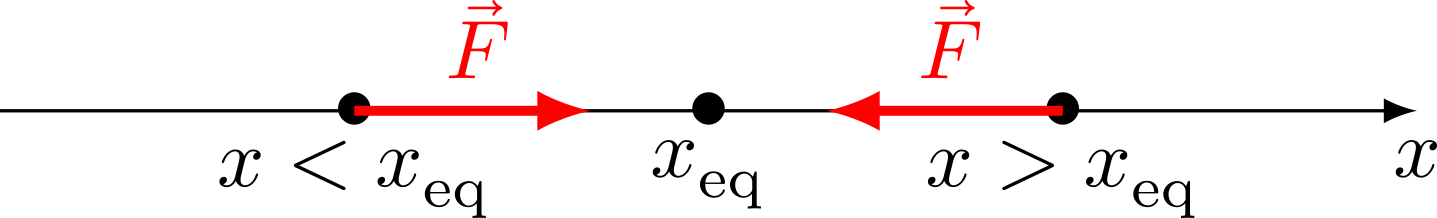
\includegraphics[width=\linewidth]{stab_a-xeq}
            \captionof{figure}{Équilibre stable}
        \end{center}
    \end{minipage}
    \hfill
    \begin{minipage}{0.45\linewidth}
        \begin{center}
            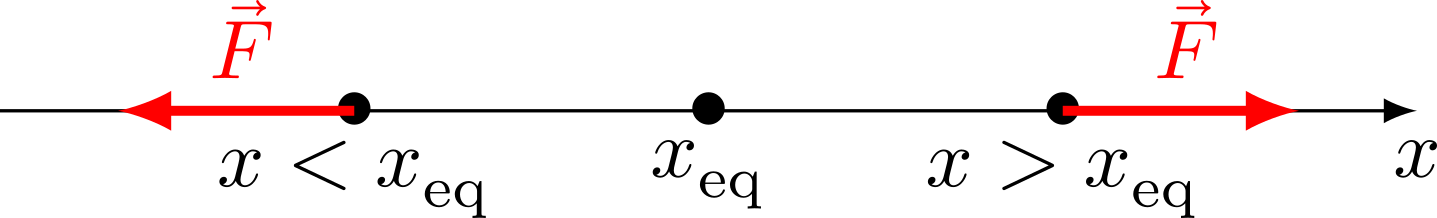
\includegraphics[width=\linewidth]{instab_a-xeq}
            \captionof{figure}{Équilibre instable}
        \end{center}
    \end{minipage}
\end{tdefi}

Pour étudier ces situations mathématiquement, on peut développer l'expression de
la somme $\Ff$ au voisinage d'un point d'équilibre $x_{\eq}$ quelconque~:
\begin{gather*}
    F(x) = F(x_{\eq}) + (x-x_{\eq})\times \eval{\dv{F}{x}}_{x_{\eq}}
    \\\Lra
    F(x) = - \eval{\dv{\Ec_p}{x}}_{x_{\eq}} -
        (x-x_{\eq})\times\eval{\dv[2]{\Ec_p}{x}}_{x_{\eq}}
\end{gather*}

Si c'est un équilibre, on a donc $F(x_{\eq}) = 0$ donc
$\eval{\dv{\Ec_p}{x}}_{x_{\eq}}$, et ainsi
\[F(x) = -(x-x_{\eq}) \eval{\dv[2]{\Ec_p}{x}}_{x_{\eq}}\]

\begin{itemize}
    \item Si c'est un équilibre \textbf{stable}, la force doit \textbf{ramener}
        le point $x$ vers sa position d'équilibre~; ainsi par exemple
        \begin{gather*}
            (x-x_{\eq}) > 0 \Ra F < 0
            \\\Lra
            \eval{\dv[2]{\Ec_p}{x}}_{x_{\eq}} > 0
        \end{gather*}
        et si $(x-x_{\eq}) < 0$, alors $F$ doit être $>0$, mais la conclusion
        est la même.
    \item Si c'est un équilibre \textbf{instable}, la force doit
        l'\textbf{écarter} de la position d'équilibre~; ainsi par exemple
        \begin{gather*}
            (x-x_{\eq}) > 0 \Ra F > 0
            \\\Lra
            \eval{\dv[2]{\Ec_p}{x}}_{x_{\eq}} < 0
        \end{gather*}
        et si $(x-x_{\eq}) < 0$, alors $F$ doit être $<0$, mais la conclusion
        est la même.
\end{itemize}

Le raisonnement se propage dans toutes les directions, on peut donc utiliser le
cas général à trois dimensions~:

\begin{tprop}{Propriété, heart}
    Une position d'équilibre est~:\\
    \begin{rsideprop}
        \[\text{\textbf{Stable} si}
        \qquad
        \boxed{\eval{\pdv[2]{\Ec_p}{x}}_{x_{\eq}} > 0}\]
        \begin{center}
            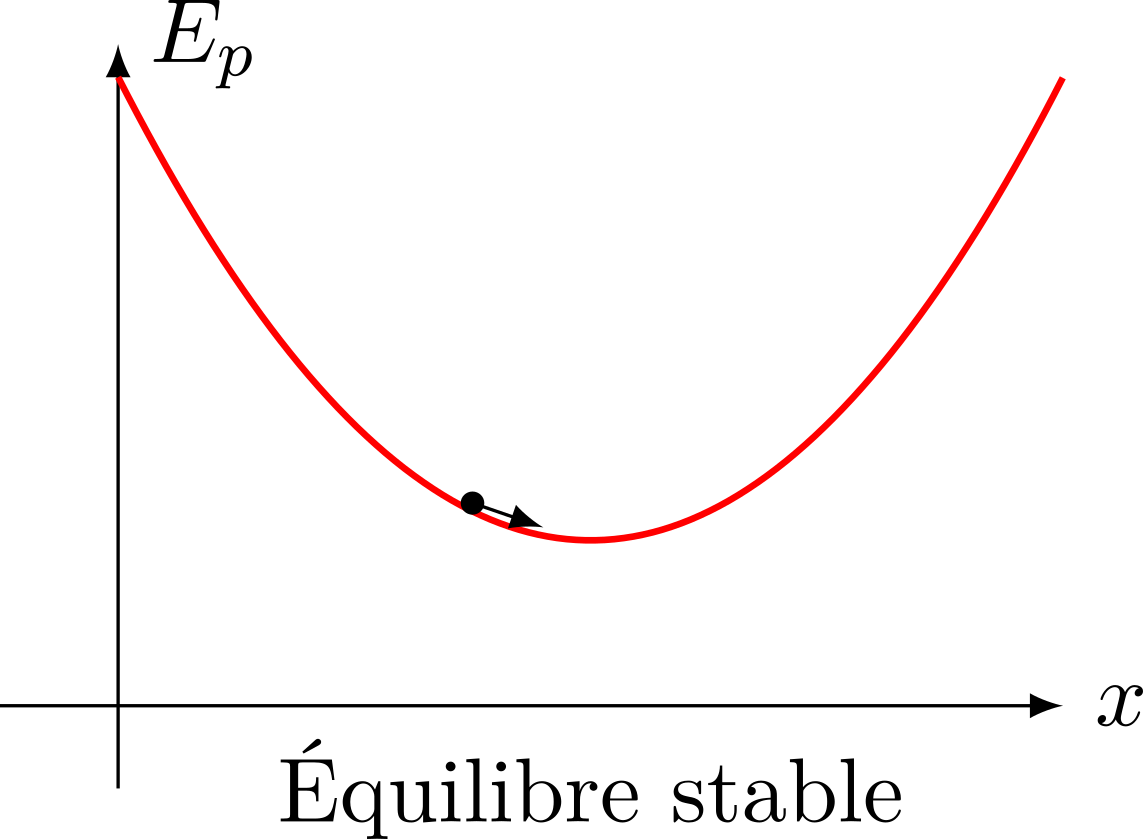
\includegraphics[width=6cm]{stab_b}
        \end{center}
        \tcblower
        \[\text{\textbf{Instable} si}
        \qquad
        \boxed{\eval{\pdv[2]{\Ec_p}{x}}_{x_{\eq}} < 0}\]
        \begin{center}
            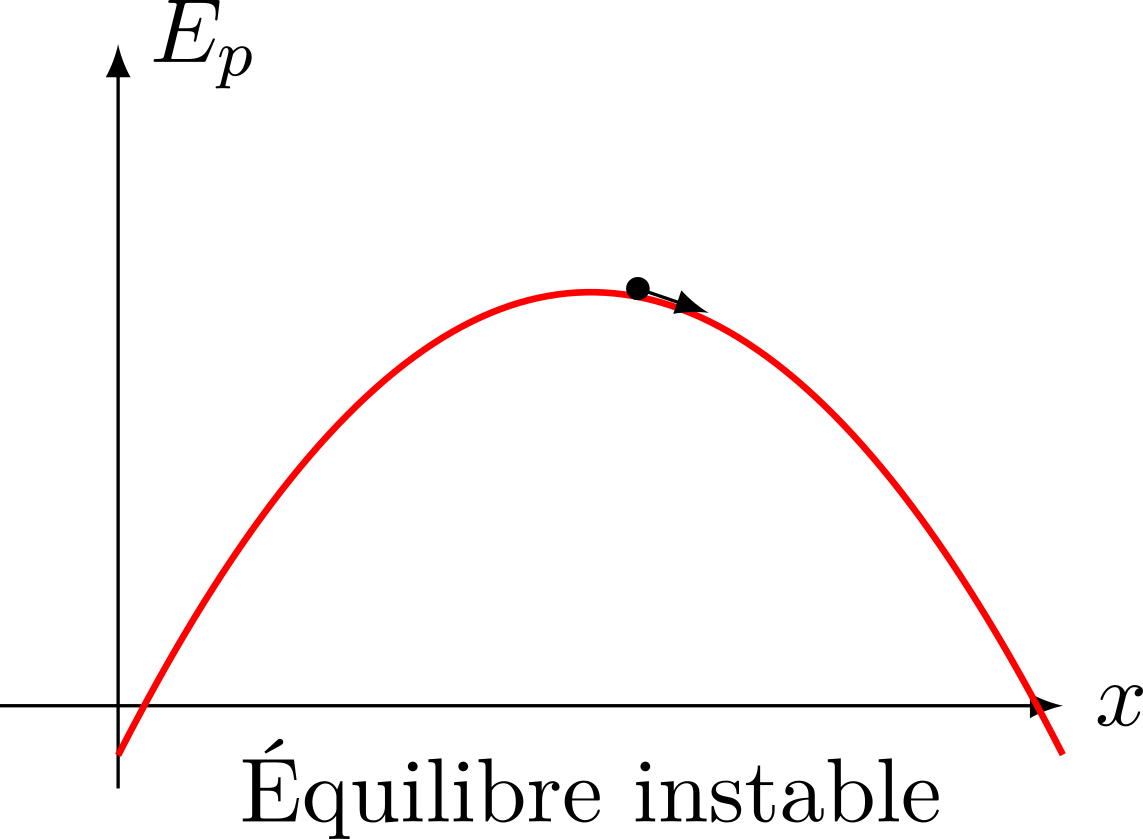
\includegraphics[width=6cm]{instab_b}
        \end{center}
    \end{rsideprop}
\end{tprop}

\begin{rexem}{Application}
    Trouver la position d'équilibre d'un ressort. Est-elle stable ou instable~?
    \tcblower
    \begin{minipage}{0.25\linewidth}
        \begin{center}
            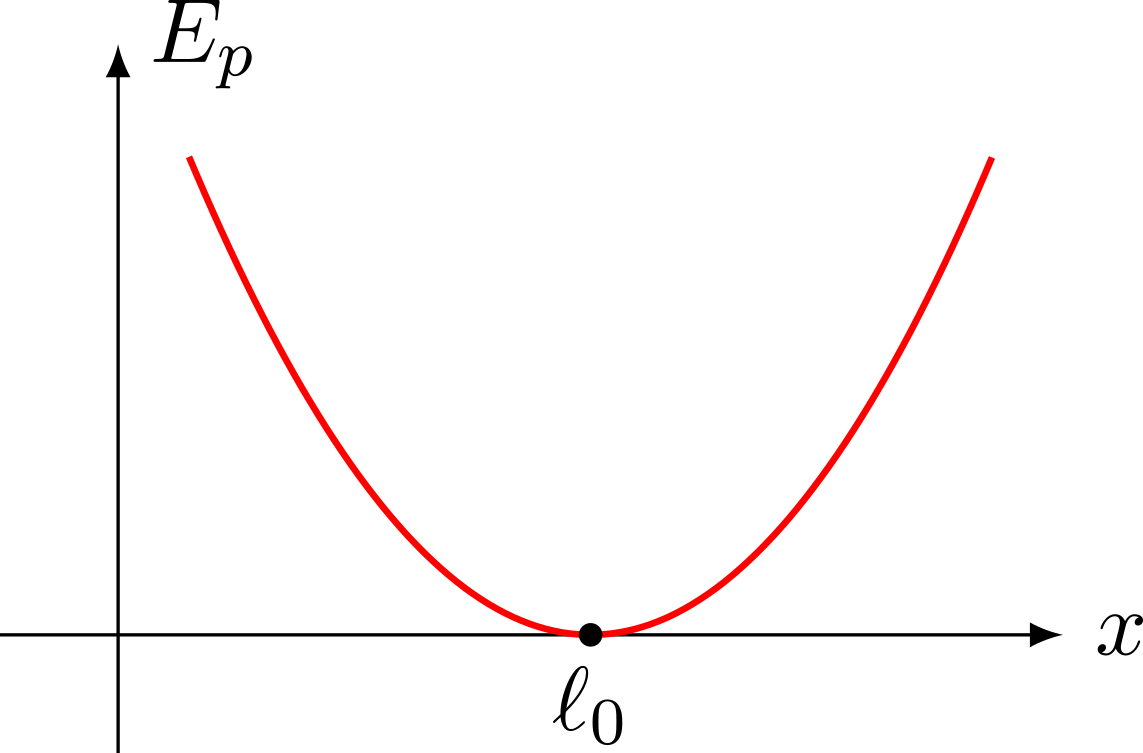
\includegraphics[width=\linewidth]{stab_ressort}
        \end{center}
    \end{minipage}
    \hfill
    \begin{minipage}{0.70\linewidth}
        L'énergie potentielle d'un ressort est
        \[
            \Ec_{p,\rm el} = \frac{1}{2}k(x-\ell_0)^2
            \Ra
            \dv{\Ec_{p,\rm el}}{x} = k(x-\ell_0)
            \Ra
            \dv[2]{\Ec_{p,\rm el}}{x} = k > 0
        \]
        Ainsi, la position d'équilibre est en $x_{\eq} = \ell_0$, et elle est
        stable.
    \end{minipage}
\end{rexem}

\subsection{Étude générale au voisinage d'un point d'équilibre stable}
En faisant un développement limité de l'énergie potentielle d'un système autour
d'une position d'équilibre stable, on a
\begin{gather*}
    \Ec_p(x) = \Ec_p(x_{\eq}) +
    \underbrace{\eval{\pdv{\Ec_p}{x}}_{x_{\eq}}}_{=0} +
    \frac{(x-x_0)^2}{2}\eval{\pdv[2]{\Ec_p}{x}}_{x_{\eq}}
\end{gather*}
\leftcenters{Notons}{$\boxed{\DS k = \eval{\pdv[2]{\Ec_p}{x}}_{x_{\eq}}}$}
\smallbreak\noindent
Alors,
\[\Ec_m = \Ec_c + \Ec_p = \frac{1}{2}m\xp^2 + \frac{1}{2}k(x-x_0)^2\]
Et si l'énergie mécanique se conserve, on a $\dv{\Ec_m}{t} = 0$ donc
\begin{gather*}
    \frac{1}{2}m(2\xpp\xp) + \frac{1}{2}k 2\xp(x-x_{\eq}) = 0
    \\\Lra
    \boxed{\xpp + \frac{k}{m}(x-x_{\eq}) = 0}
\end{gather*}

On retrouve l'équation de l'oscillateur harmonique~! Le mobile oscille autour de
la position d'équilibre à la pulsation $\w_0 = \sqrt{k/m}$ avec $k =
\eval{\pdv[2]{\Ec_p}{x}}_{x_{\eq}}$. Ce qui est phénoménal, c'est que \textbf{la
seule supposition est que le système soit conservatif}. Ceci explique
l'abondance des systèmes harmoniques dans la nature.

\begin{rrema}{Remarque}
    Si l'équilibre est instable, on prend
    \[k = - \eval{\pdv[2]{\Ec_p}{x}}_{x_{\eq}} > 0\]
    d'où par le même raisonnement,
    \[\xpp - \frac{k}{m}(x-x_{\eq}) = 0\]
    de solution
    \[x-x_{\eq} = A\exr^{\w_0t} + B^{-\w_0t}\]
    Et pour un écart $x_0$ de la position d'équilibre sans vitesse initiale, on
    a
    \[x - x_{\eq} = x_0\cosh(\w_0t)\]
    donc proche d'un point d'équilibre instable, le mobile s'écarte
    exponentiellement de cette position.
\end{rrema}

\section{Énergie potentielle et trajectoire}


\subsection{Détermination qualitative d'une trajectoire}
Pour un point matériel soumis seulement à des forces conservatives (ou ne
travaillant pas), il est possible de prévoir les zones accessibles au mobile
ainsi que l'aspect de la trajectoire en étudiant l'énergie potentielle. En
effet,
\[\Ec_m = \Ec_c + \Ec_p \geq \Ec_p\]
puisque l'énergie cinétique est positive. Ainsi~:
\begin{tror}{Trajectoire et énergie potentielle, heart}
    Dans un diagramme d'énergie potentielle selon $x$~:
    \begin{itemize}
        \item Seules les régions où $\Ec_p \leq \Ec_m$ sont accessibles~;
        \item Lorsque $\Ec_p = \Ec_m$, $\Ec_c = 0$ donc la vitesse est nulle~;
        \item Lorsque $\Ec_p$ est minimale, $\Ec_c$ est maximale donc la vitesse
            est maximale
        % \item Si les valeurs de $x$ sont \textbf{bornées}, on dit que le système
        %     est dans un \textbf{état lié}~;
        % \item Si les valeurs de $x$ peuvent tendre vers \textbf{l'infini}, le
        %     système est dans un \textbf{état de diffusion}
    \end{itemize}\bigbreak
    \begin{minipage}{0.47\linewidth}
        \begin{center}
            \bfseries
            \fbox{État lié}
        \end{center}
        La particule reste dans une zone bornée de l’espace et le mobile effectue
        des aller-retours périodiques autour de la position d’équilibre.
        \begin{center}
            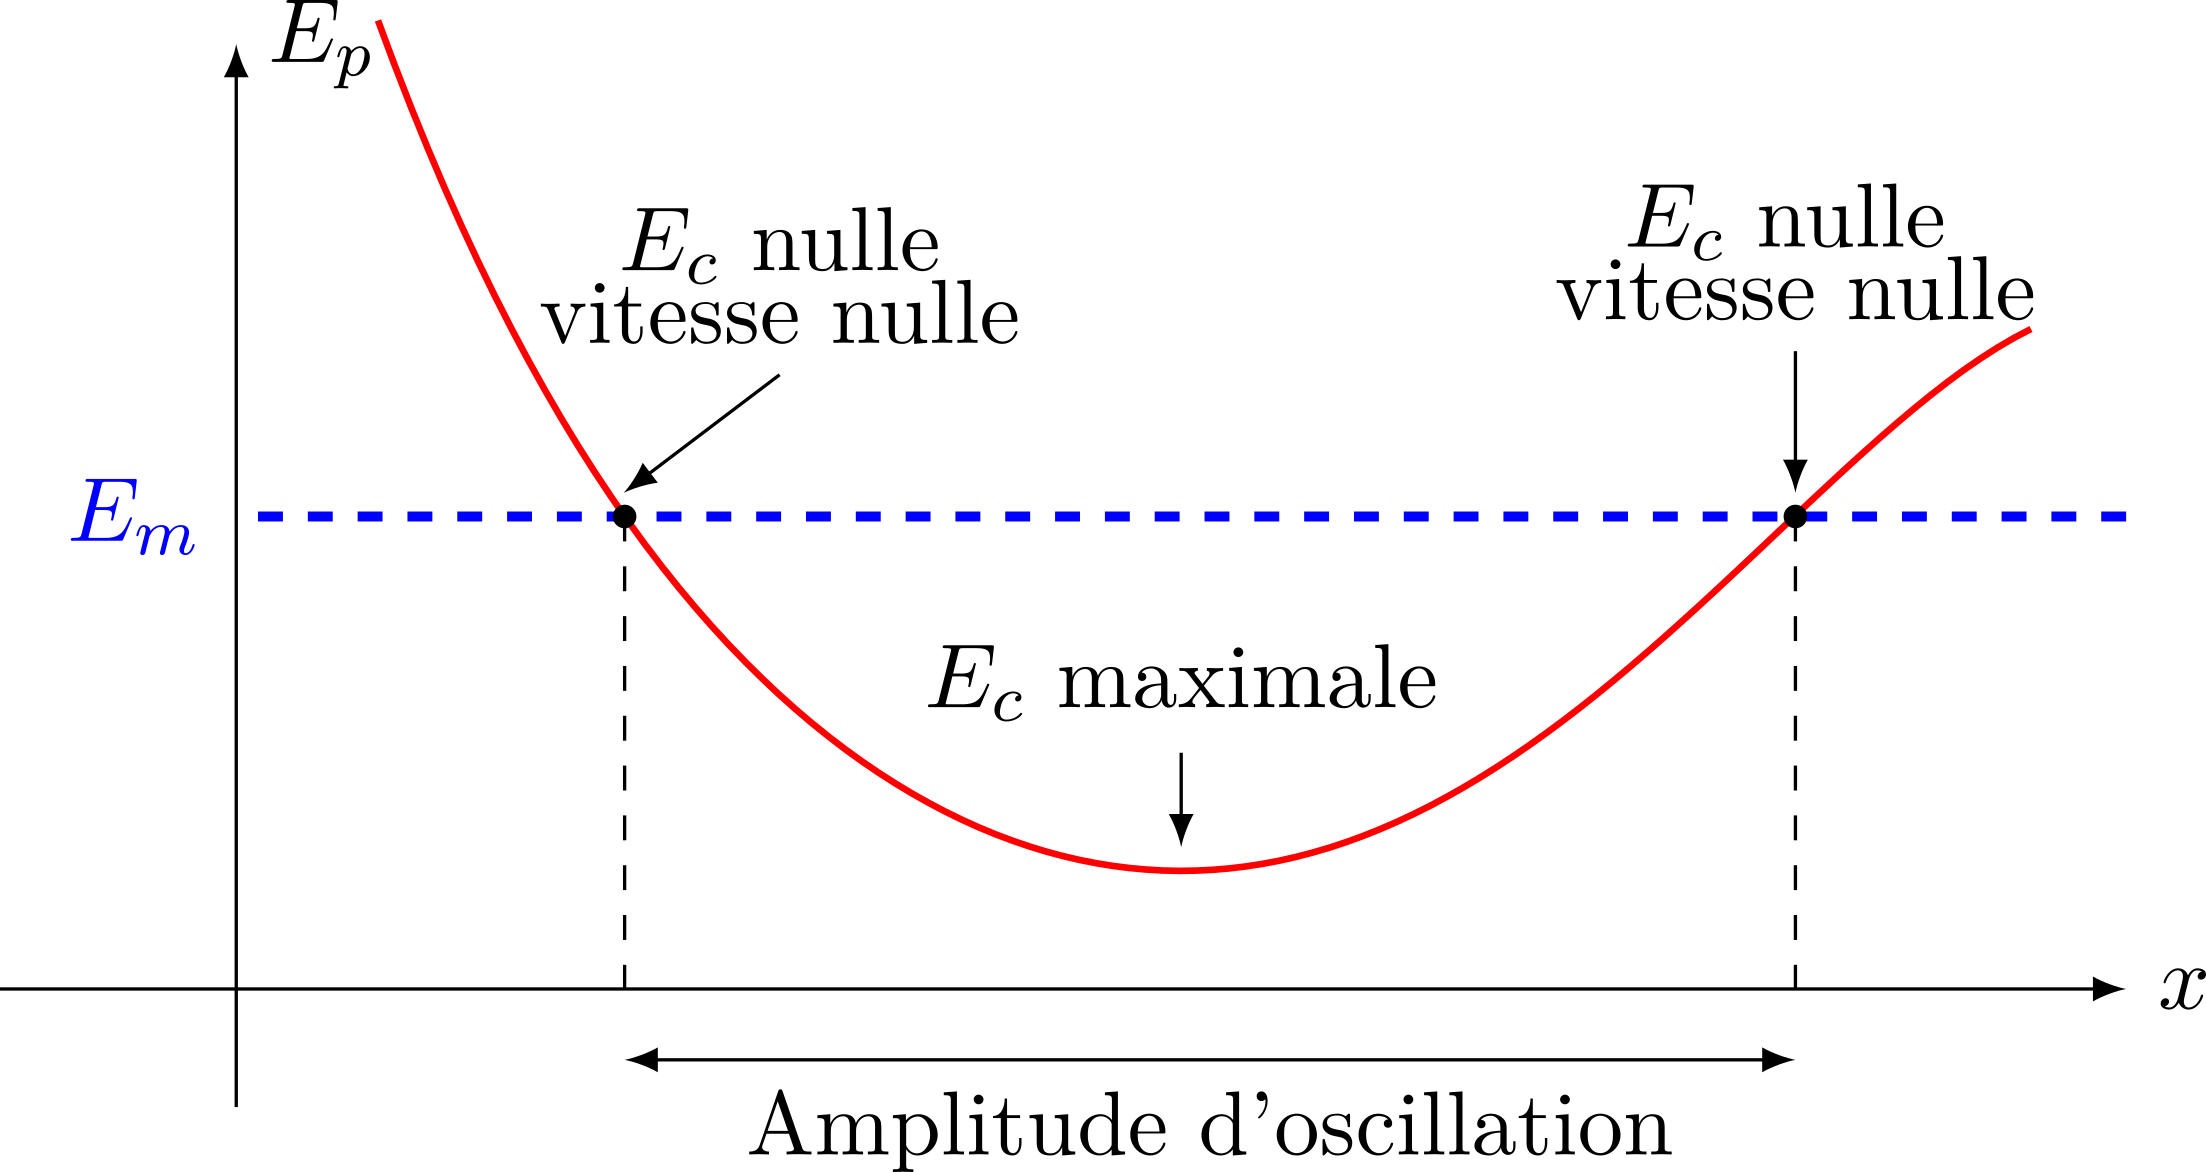
\includegraphics[width=7cm]{stab_lie}
        \end{center}
    \end{minipage}
    \hfill
    \begin{minipage}{0.47\linewidth}
        \begin{center}
            \bfseries
            \fbox{État de diffusion}
        \end{center}
        La particule aura tendance à partir vers $x = +\infty$ sans jamais revenir :
        son mouvement n’est pas borné dans l’espace.
        \begin{center}
            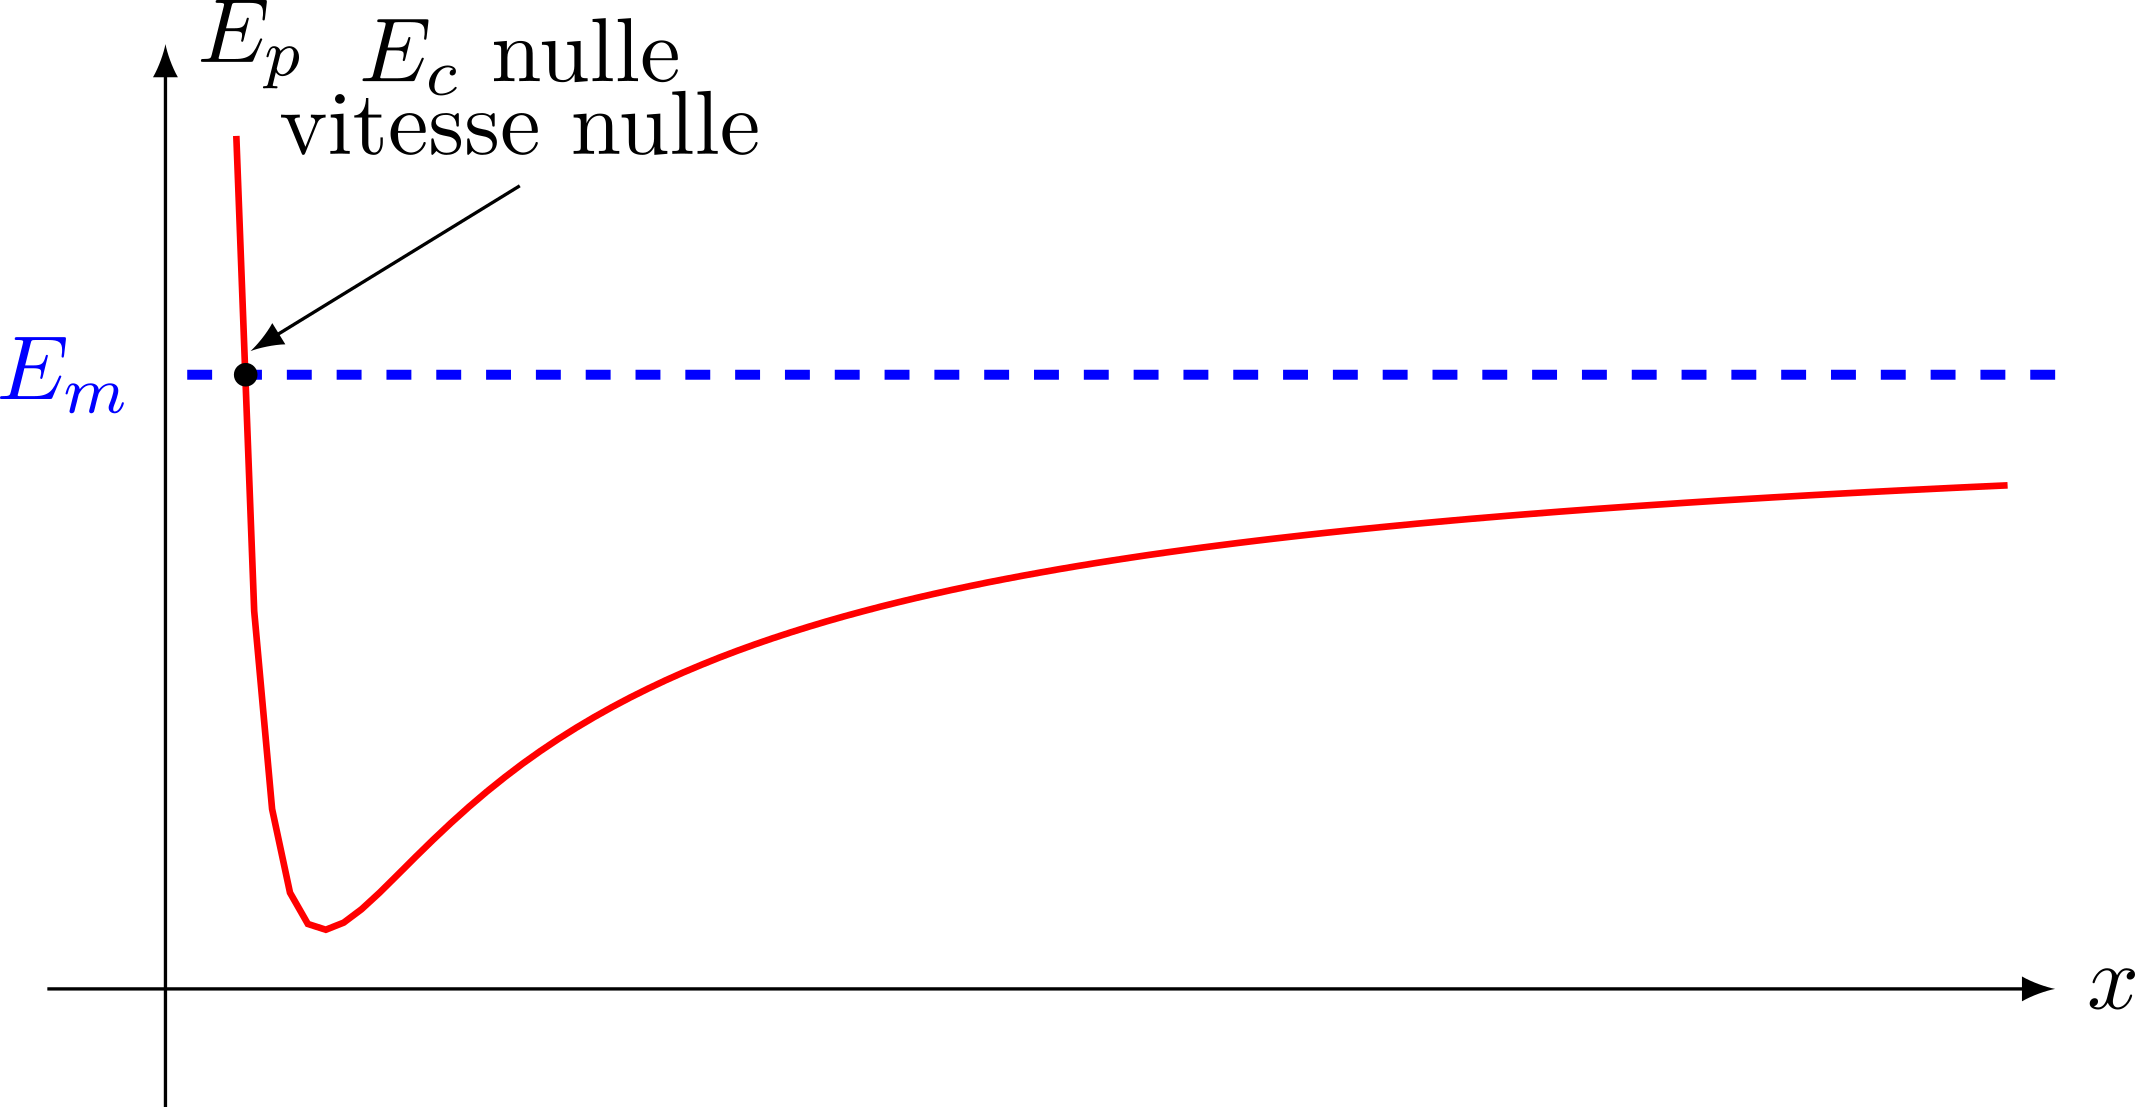
\includegraphics[width=7cm]{stab_diff}
        \end{center}
    \end{minipage}
\end{tror}

Certains corps célestes sont dans des états liés, comme la Terre et le Soleil,
d'autres dans des états de diffusion~: ils passent brièvement dans le système
solaire avant de le quitter définitivement. C'est le cas de la comète
d'\textsc{Arend-Roland}, passée à proximité de la Terre en 1956 mais qui ne
devrait jamais revenir.

\subsection{Cas du pendule simple}
On reprend le pendule simple, que l'on suppose attaché avec une tige
\textbf{rigide} (pour éviter les décrochages). On souhaiterait déterminer ses
positions d'équilibre et étudier ses trajectoires possibles. Le système étant
conservatif ($\Pf$ conservatif et $\Tf\perp\vf$), déterminons l'expression de
l'énergie potentielle en fonction de l'angle.

\leftcenters{L'altitude est~:}{$z(\tt) = \ell(1-\cos\tt)$}
\smallbreak\noindent
\leftcenters{donc l'énergie potentielle est}{$\boxed{\Ec_p(\tt) = mgz(\tt) =
mg\ell(1-\cos\tt)}$}
\begin{center}
    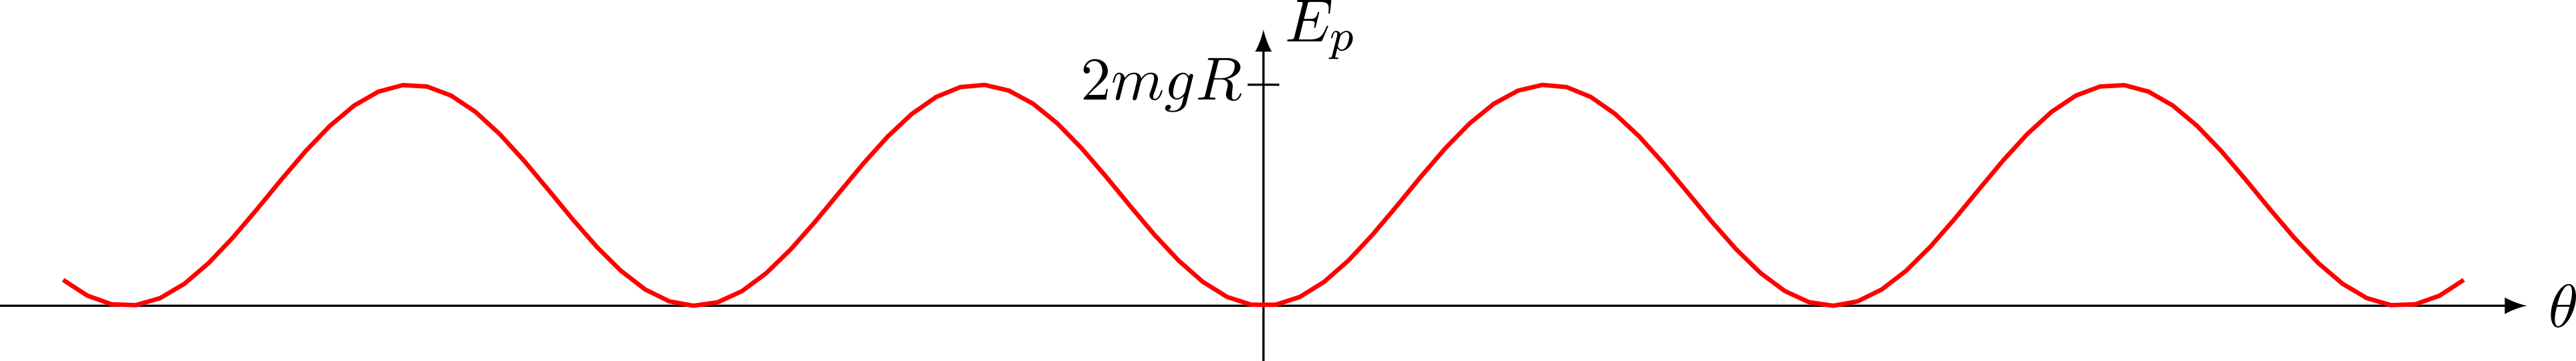
\includegraphics[scale=1]{stab_pend-a}
\end{center}
Les positions d'équilibre stables sont donc celles dans les «~creux~», soit $\tt =
2p\pi$ avec $p\in\Zb$, et les instables sur les «~collines~», soit $\tt =
(2p+1)\pi$. On distingue alors deux cas~:

\subsubsection{Cas $\Ec_m < 2mg\ell$}
Si l'énergie mécanique totale est inférieure à l'énergie potentielle maximale, on se
situera dans un état lié, «~coincé~» dans un creux. On observera donc une
oscillation autour du point d'équilibre le plus proche, et on a vu que cette
oscillation état sinusoïdale aux très petits angles ($\abs{\tt} < \ang{20}$).

\begin{minipage}{0.45\linewidth}
    \begin{center}
        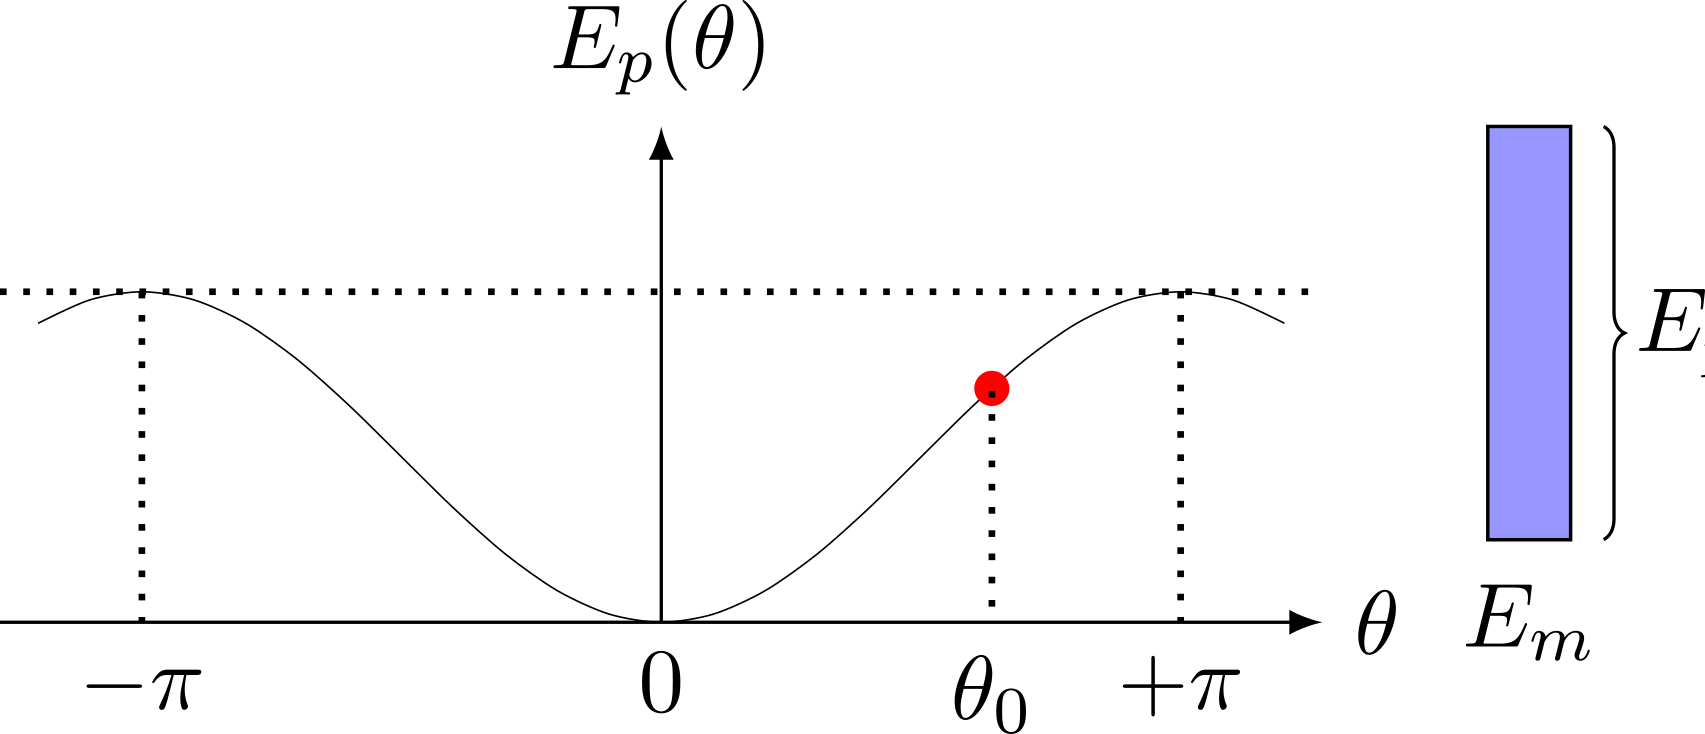
\includegraphics[width=7cm]{stab_pend-b}
        \captionof{figure}{État initial $\tt = \tt_0$~: toute l'énergie est sous
        forme d'énergie potentielle, et l'énergie est nulle.}
    \end{center}
\end{minipage}
\hfill
\begin{minipage}{0.45\linewidth}
    \begin{center}
        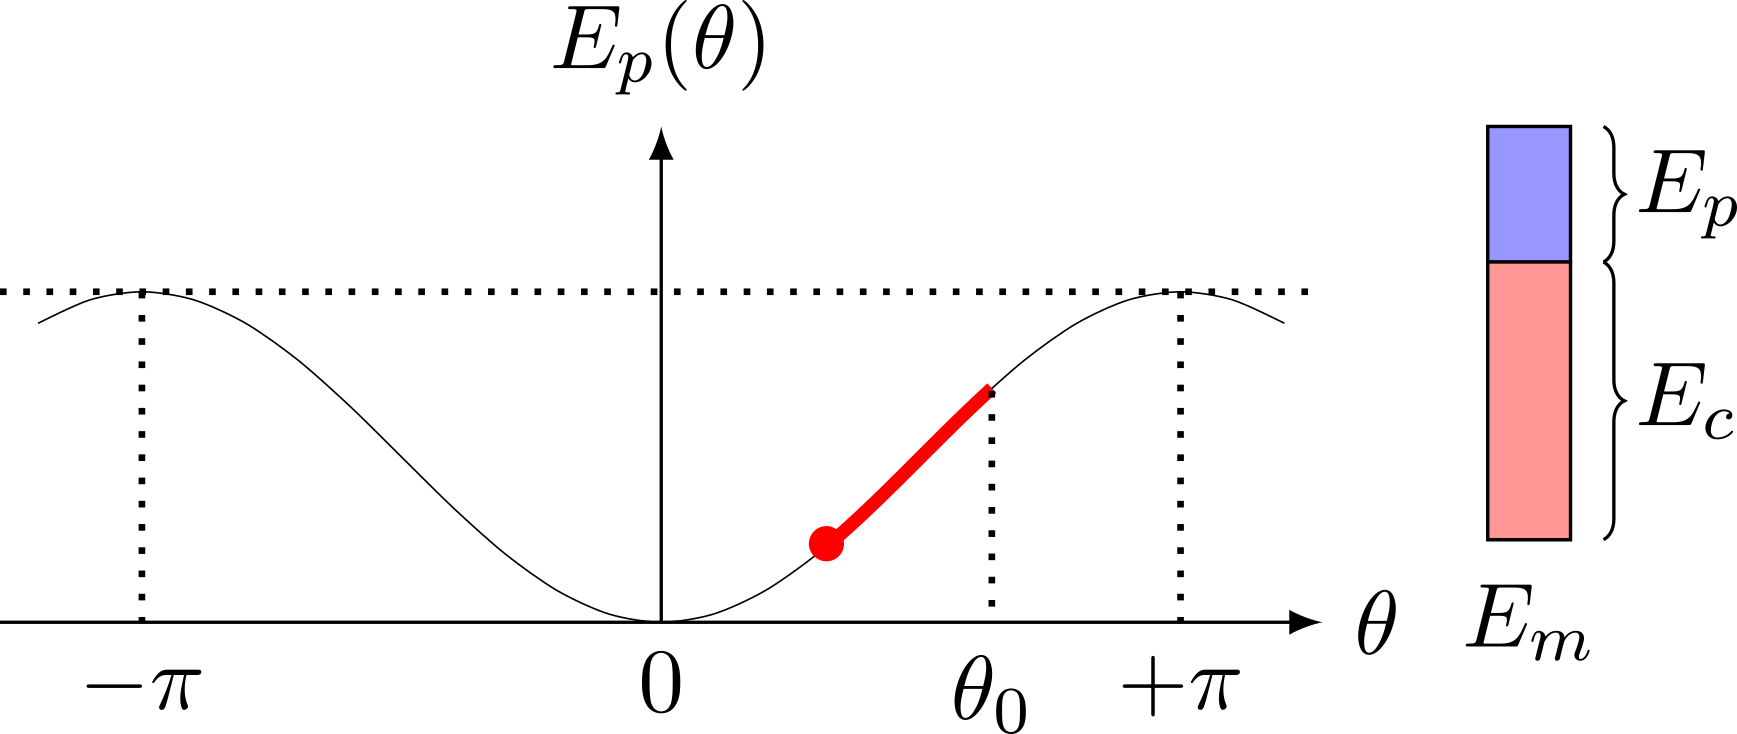
\includegraphics[width=7cm]{stab_pend-c}
        \captionof{figure}{La masse perd de l'énergie potentielle tout en restant sur
        la courbe. L'énergie mécanique étant conservée, elle gagne de l'énergie
    cinétique et donc de la vitesse.}
    \end{center}
\end{minipage}

\begin{minipage}{0.45\linewidth}
    \begin{center}
        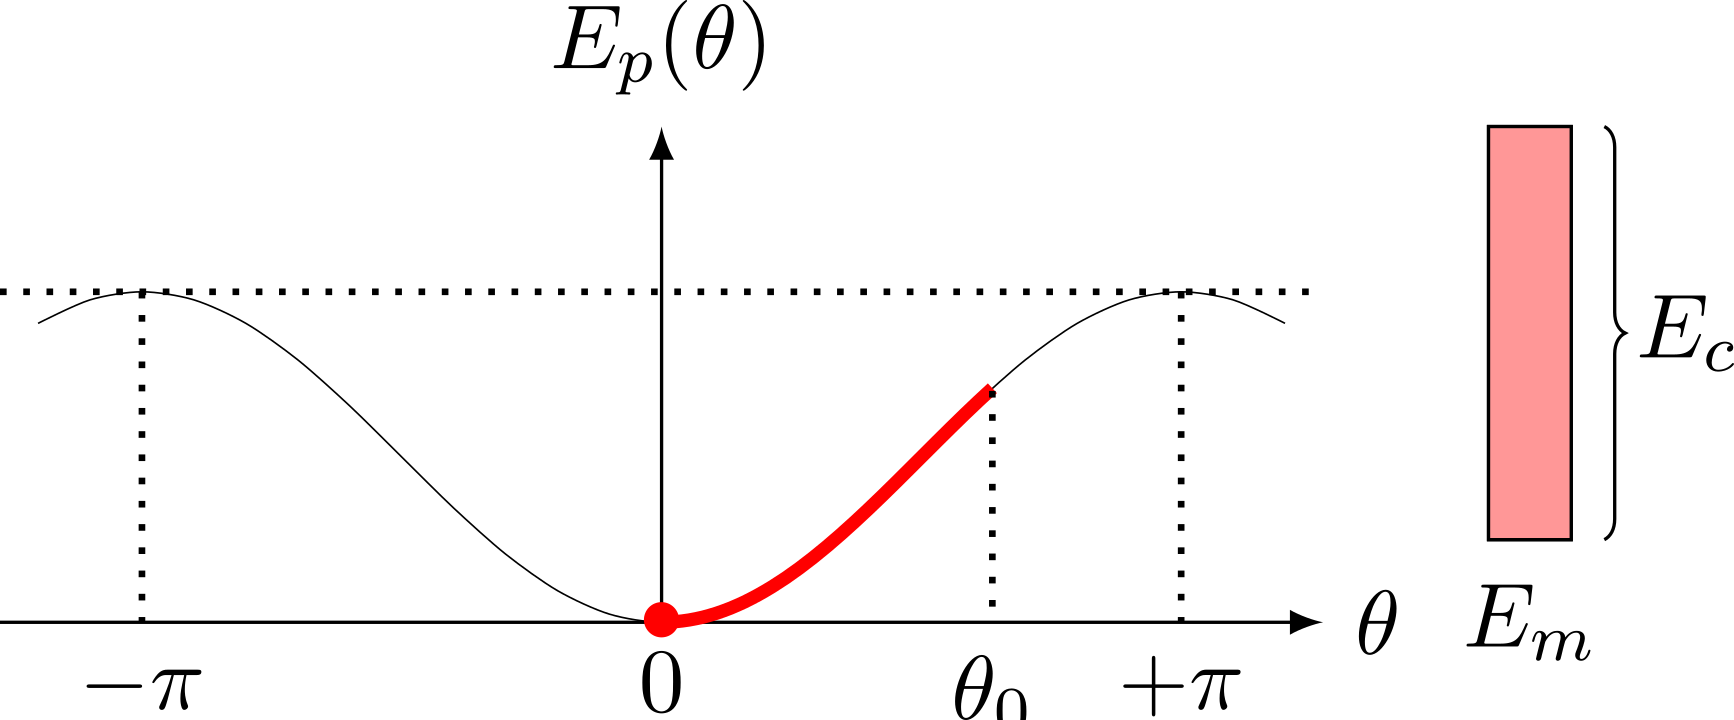
\includegraphics[width=7cm]{stab_pend-d}
        \captionof{figure}{La masse a perdu toute son énergie potentielle~: son
        énergie cinétique et donc sa vitesse sont maximales.}
    \end{center}
\end{minipage}
\hfill
\begin{minipage}{0.45\linewidth}
    \begin{center}
        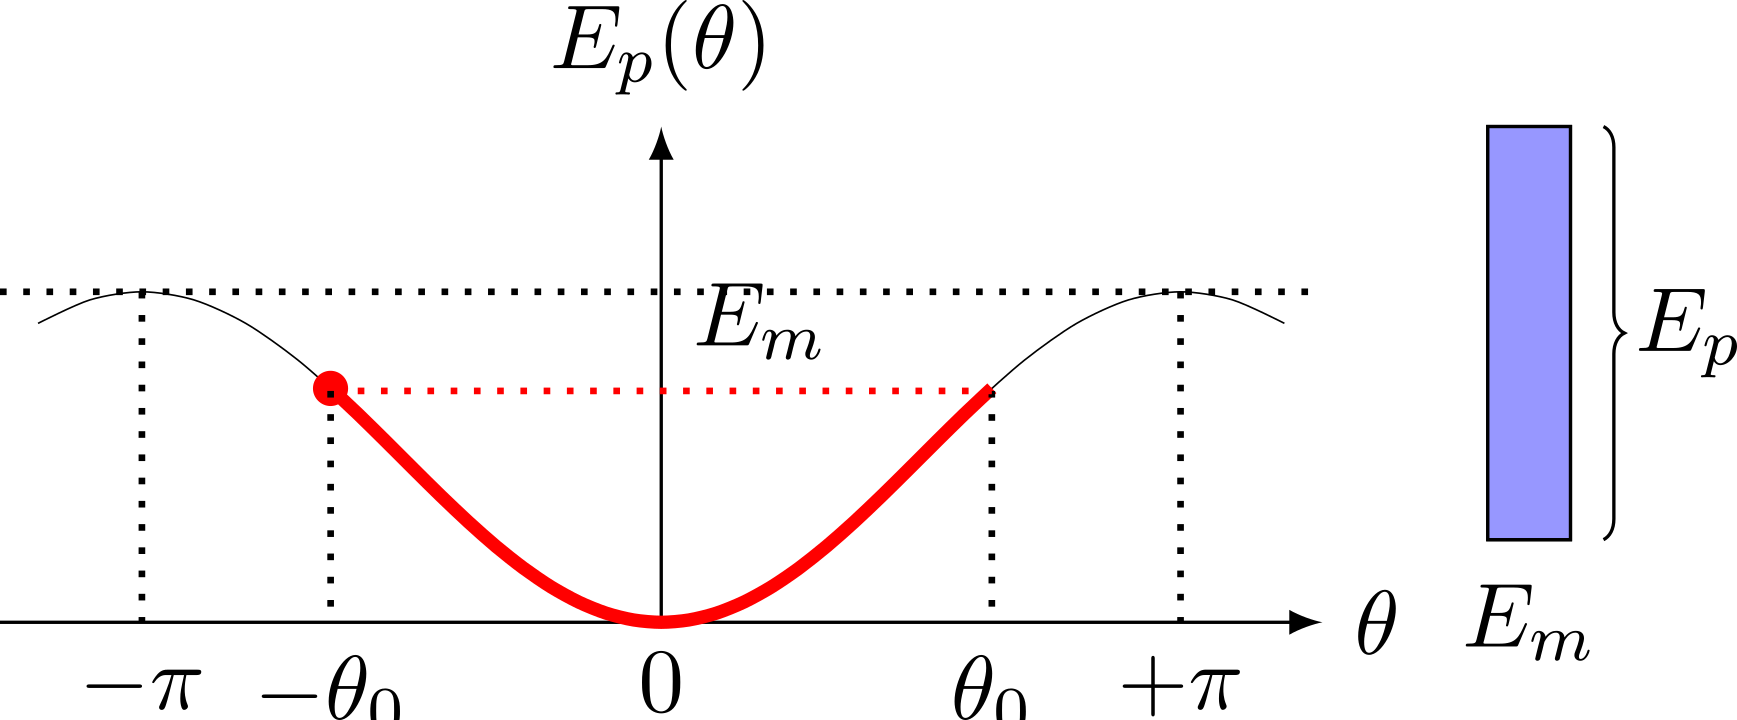
\includegraphics[width=7cm]{stab_pend-e}
        \captionof{figure}{La masse a perdu toute son énergie cinétique et a
        maximisé son énergie potentielle. Elle a atteint l'angle maximale
    $-\tt_0$, et repart dans l'autre sens.}
    \end{center}
\end{minipage}

\vspace{-15pt}
\subsubsection{Cas $\Ec_m > 2mg\ell$}
Si l'énergie mécanique totale est supérieure à l'énergie potentielle maximale,
ça veut dire qu'il y a un excédent d'énergie cinétique. Ainsi, le pendule tourne
autour de l'axe de rotation, et lorsqu'il arrive en $\tt = \pi$ l'énergie
potentielle est maximale mais l'énergie cinétique n'est pas nulle~: il continue
sa rotation, sans oscillation. La vitesse n'est cependant pas constante, elle
est plus faible en haut qu'en bas du mouvement (par conservation de l'énergie
mécanique).

Une animation est disponible en
ligne\footnote{\url{https://phyanim.sciences.univ-nantes.fr/Meca/Oscillateurs/tension_pendule.php}}.

\end{document}
